
% Default to the notebook output style

    


% Inherit from the specified cell style.




    
\documentclass[11pt]{article}

    
    
    \usepackage[T1]{fontenc}
    % Nicer default font than Computer Modern for most use cases
    \usepackage{palatino}

    % Basic figure setup, for now with no caption control since it's done
    % automatically by Pandoc (which extracts ![](path) syntax from Markdown).
    \usepackage{graphicx}
    % We will generate all images so they have a width \maxwidth. This means
    % that they will get their normal width if they fit onto the page, but
    % are scaled down if they would overflow the margins.
    \makeatletter
    \def\maxwidth{\ifdim\Gin@nat@width>\linewidth\linewidth
    \else\Gin@nat@width\fi}
    \makeatother
    \let\Oldincludegraphics\includegraphics
    % Set max figure width to be 80% of text width, for now hardcoded.
    \renewcommand{\includegraphics}[1]{\Oldincludegraphics[width=.8\maxwidth]{#1}}
    % Ensure that by default, figures have no caption (until we provide a
    % proper Figure object with a Caption API and a way to capture that
    % in the conversion process - todo).
    \usepackage{caption}
    \DeclareCaptionLabelFormat{nolabel}{}
    \captionsetup{labelformat=nolabel}

    \usepackage{adjustbox} % Used to constrain images to a maximum size 
    \usepackage{xcolor} % Allow colors to be defined
    \usepackage{enumerate} % Needed for markdown enumerations to work
    \usepackage{geometry} % Used to adjust the document margins
    \usepackage{amsmath} % Equations
    \usepackage{amssymb} % Equations
    \usepackage{textcomp} % defines textquotesingle
    % Hack from http://tex.stackexchange.com/a/47451/13684:
    \AtBeginDocument{%
        \def\PYZsq{\textquotesingle}% Upright quotes in Pygmentized code
    }
    \usepackage{upquote} % Upright quotes for verbatim code
    \usepackage{eurosym} % defines \euro
    \usepackage[mathletters]{ucs} % Extended unicode (utf-8) support
    \usepackage[utf8x]{inputenc} % Allow utf-8 characters in the tex document
    \usepackage{fancyvrb} % verbatim replacement that allows latex
    \usepackage{grffile} % extends the file name processing of package graphics 
                         % to support a larger range 
    % The hyperref package gives us a pdf with properly built
    % internal navigation ('pdf bookmarks' for the table of contents,
    % internal cross-reference links, web links for URLs, etc.)
    \usepackage{hyperref}
    \usepackage{longtable} % longtable support required by pandoc >1.10
    \usepackage{booktabs}  % table support for pandoc > 1.12.2
    \usepackage[normalem]{ulem} % ulem is needed to support strikethroughs (\sout)
                                % normalem makes italics be italics, not underlines
    

    
    
    % Colors for the hyperref package
    \definecolor{urlcolor}{rgb}{0,.145,.698}
    \definecolor{linkcolor}{rgb}{.71,0.21,0.01}
    \definecolor{citecolor}{rgb}{.12,.54,.11}

    % ANSI colors
    \definecolor{ansi-black}{HTML}{3E424D}
    \definecolor{ansi-black-intense}{HTML}{282C36}
    \definecolor{ansi-red}{HTML}{E75C58}
    \definecolor{ansi-red-intense}{HTML}{B22B31}
    \definecolor{ansi-green}{HTML}{00A250}
    \definecolor{ansi-green-intense}{HTML}{007427}
    \definecolor{ansi-yellow}{HTML}{DDB62B}
    \definecolor{ansi-yellow-intense}{HTML}{B27D12}
    \definecolor{ansi-blue}{HTML}{208FFB}
    \definecolor{ansi-blue-intense}{HTML}{0065CA}
    \definecolor{ansi-magenta}{HTML}{D160C4}
    \definecolor{ansi-magenta-intense}{HTML}{A03196}
    \definecolor{ansi-cyan}{HTML}{60C6C8}
    \definecolor{ansi-cyan-intense}{HTML}{258F8F}
    \definecolor{ansi-white}{HTML}{C5C1B4}
    \definecolor{ansi-white-intense}{HTML}{A1A6B2}

    % commands and environments needed by pandoc snippets
    % extracted from the output of `pandoc -s`
    \providecommand{\tightlist}{%
      \setlength{\itemsep}{0pt}\setlength{\parskip}{0pt}}
    \DefineVerbatimEnvironment{Highlighting}{Verbatim}{commandchars=\\\{\}}
    % Add ',fontsize=\small' for more characters per line
    \newenvironment{Shaded}{}{}
    \newcommand{\KeywordTok}[1]{\textcolor[rgb]{0.00,0.44,0.13}{\textbf{{#1}}}}
    \newcommand{\DataTypeTok}[1]{\textcolor[rgb]{0.56,0.13,0.00}{{#1}}}
    \newcommand{\DecValTok}[1]{\textcolor[rgb]{0.25,0.63,0.44}{{#1}}}
    \newcommand{\BaseNTok}[1]{\textcolor[rgb]{0.25,0.63,0.44}{{#1}}}
    \newcommand{\FloatTok}[1]{\textcolor[rgb]{0.25,0.63,0.44}{{#1}}}
    \newcommand{\CharTok}[1]{\textcolor[rgb]{0.25,0.44,0.63}{{#1}}}
    \newcommand{\StringTok}[1]{\textcolor[rgb]{0.25,0.44,0.63}{{#1}}}
    \newcommand{\CommentTok}[1]{\textcolor[rgb]{0.38,0.63,0.69}{\textit{{#1}}}}
    \newcommand{\OtherTok}[1]{\textcolor[rgb]{0.00,0.44,0.13}{{#1}}}
    \newcommand{\AlertTok}[1]{\textcolor[rgb]{1.00,0.00,0.00}{\textbf{{#1}}}}
    \newcommand{\FunctionTok}[1]{\textcolor[rgb]{0.02,0.16,0.49}{{#1}}}
    \newcommand{\RegionMarkerTok}[1]{{#1}}
    \newcommand{\ErrorTok}[1]{\textcolor[rgb]{1.00,0.00,0.00}{\textbf{{#1}}}}
    \newcommand{\NormalTok}[1]{{#1}}
    
    % Additional commands for more recent versions of Pandoc
    \newcommand{\ConstantTok}[1]{\textcolor[rgb]{0.53,0.00,0.00}{{#1}}}
    \newcommand{\SpecialCharTok}[1]{\textcolor[rgb]{0.25,0.44,0.63}{{#1}}}
    \newcommand{\VerbatimStringTok}[1]{\textcolor[rgb]{0.25,0.44,0.63}{{#1}}}
    \newcommand{\SpecialStringTok}[1]{\textcolor[rgb]{0.73,0.40,0.53}{{#1}}}
    \newcommand{\ImportTok}[1]{{#1}}
    \newcommand{\DocumentationTok}[1]{\textcolor[rgb]{0.73,0.13,0.13}{\textit{{#1}}}}
    \newcommand{\AnnotationTok}[1]{\textcolor[rgb]{0.38,0.63,0.69}{\textbf{\textit{{#1}}}}}
    \newcommand{\CommentVarTok}[1]{\textcolor[rgb]{0.38,0.63,0.69}{\textbf{\textit{{#1}}}}}
    \newcommand{\VariableTok}[1]{\textcolor[rgb]{0.10,0.09,0.49}{{#1}}}
    \newcommand{\ControlFlowTok}[1]{\textcolor[rgb]{0.00,0.44,0.13}{\textbf{{#1}}}}
    \newcommand{\OperatorTok}[1]{\textcolor[rgb]{0.40,0.40,0.40}{{#1}}}
    \newcommand{\BuiltInTok}[1]{{#1}}
    \newcommand{\ExtensionTok}[1]{{#1}}
    \newcommand{\PreprocessorTok}[1]{\textcolor[rgb]{0.74,0.48,0.00}{{#1}}}
    \newcommand{\AttributeTok}[1]{\textcolor[rgb]{0.49,0.56,0.16}{{#1}}}
    \newcommand{\InformationTok}[1]{\textcolor[rgb]{0.38,0.63,0.69}{\textbf{\textit{{#1}}}}}
    \newcommand{\WarningTok}[1]{\textcolor[rgb]{0.38,0.63,0.69}{\textbf{\textit{{#1}}}}}
    
    
    % Define a nice break command that doesn't care if a line doesn't already
    % exist.
    \def\br{\hspace*{\fill} \\* }
    % Math Jax compatability definitions
    \def\gt{>}
    \def\lt{<}
    % Document parameters
    \title{Homework 2}
    
    
    

    % Pygments definitions
    
\makeatletter
\def\PY@reset{\let\PY@it=\relax \let\PY@bf=\relax%
    \let\PY@ul=\relax \let\PY@tc=\relax%
    \let\PY@bc=\relax \let\PY@ff=\relax}
\def\PY@tok#1{\csname PY@tok@#1\endcsname}
\def\PY@toks#1+{\ifx\relax#1\empty\else%
    \PY@tok{#1}\expandafter\PY@toks\fi}
\def\PY@do#1{\PY@bc{\PY@tc{\PY@ul{%
    \PY@it{\PY@bf{\PY@ff{#1}}}}}}}
\def\PY#1#2{\PY@reset\PY@toks#1+\relax+\PY@do{#2}}

\expandafter\def\csname PY@tok@w\endcsname{\def\PY@tc##1{\textcolor[rgb]{0.73,0.73,0.73}{##1}}}
\expandafter\def\csname PY@tok@c\endcsname{\let\PY@it=\textit\def\PY@tc##1{\textcolor[rgb]{0.25,0.50,0.50}{##1}}}
\expandafter\def\csname PY@tok@cp\endcsname{\def\PY@tc##1{\textcolor[rgb]{0.74,0.48,0.00}{##1}}}
\expandafter\def\csname PY@tok@k\endcsname{\let\PY@bf=\textbf\def\PY@tc##1{\textcolor[rgb]{0.00,0.50,0.00}{##1}}}
\expandafter\def\csname PY@tok@kp\endcsname{\def\PY@tc##1{\textcolor[rgb]{0.00,0.50,0.00}{##1}}}
\expandafter\def\csname PY@tok@kt\endcsname{\def\PY@tc##1{\textcolor[rgb]{0.69,0.00,0.25}{##1}}}
\expandafter\def\csname PY@tok@o\endcsname{\def\PY@tc##1{\textcolor[rgb]{0.40,0.40,0.40}{##1}}}
\expandafter\def\csname PY@tok@ow\endcsname{\let\PY@bf=\textbf\def\PY@tc##1{\textcolor[rgb]{0.67,0.13,1.00}{##1}}}
\expandafter\def\csname PY@tok@nb\endcsname{\def\PY@tc##1{\textcolor[rgb]{0.00,0.50,0.00}{##1}}}
\expandafter\def\csname PY@tok@nf\endcsname{\def\PY@tc##1{\textcolor[rgb]{0.00,0.00,1.00}{##1}}}
\expandafter\def\csname PY@tok@nc\endcsname{\let\PY@bf=\textbf\def\PY@tc##1{\textcolor[rgb]{0.00,0.00,1.00}{##1}}}
\expandafter\def\csname PY@tok@nn\endcsname{\let\PY@bf=\textbf\def\PY@tc##1{\textcolor[rgb]{0.00,0.00,1.00}{##1}}}
\expandafter\def\csname PY@tok@ne\endcsname{\let\PY@bf=\textbf\def\PY@tc##1{\textcolor[rgb]{0.82,0.25,0.23}{##1}}}
\expandafter\def\csname PY@tok@nv\endcsname{\def\PY@tc##1{\textcolor[rgb]{0.10,0.09,0.49}{##1}}}
\expandafter\def\csname PY@tok@no\endcsname{\def\PY@tc##1{\textcolor[rgb]{0.53,0.00,0.00}{##1}}}
\expandafter\def\csname PY@tok@nl\endcsname{\def\PY@tc##1{\textcolor[rgb]{0.63,0.63,0.00}{##1}}}
\expandafter\def\csname PY@tok@ni\endcsname{\let\PY@bf=\textbf\def\PY@tc##1{\textcolor[rgb]{0.60,0.60,0.60}{##1}}}
\expandafter\def\csname PY@tok@na\endcsname{\def\PY@tc##1{\textcolor[rgb]{0.49,0.56,0.16}{##1}}}
\expandafter\def\csname PY@tok@nt\endcsname{\let\PY@bf=\textbf\def\PY@tc##1{\textcolor[rgb]{0.00,0.50,0.00}{##1}}}
\expandafter\def\csname PY@tok@nd\endcsname{\def\PY@tc##1{\textcolor[rgb]{0.67,0.13,1.00}{##1}}}
\expandafter\def\csname PY@tok@s\endcsname{\def\PY@tc##1{\textcolor[rgb]{0.73,0.13,0.13}{##1}}}
\expandafter\def\csname PY@tok@sd\endcsname{\let\PY@it=\textit\def\PY@tc##1{\textcolor[rgb]{0.73,0.13,0.13}{##1}}}
\expandafter\def\csname PY@tok@si\endcsname{\let\PY@bf=\textbf\def\PY@tc##1{\textcolor[rgb]{0.73,0.40,0.53}{##1}}}
\expandafter\def\csname PY@tok@se\endcsname{\let\PY@bf=\textbf\def\PY@tc##1{\textcolor[rgb]{0.73,0.40,0.13}{##1}}}
\expandafter\def\csname PY@tok@sr\endcsname{\def\PY@tc##1{\textcolor[rgb]{0.73,0.40,0.53}{##1}}}
\expandafter\def\csname PY@tok@ss\endcsname{\def\PY@tc##1{\textcolor[rgb]{0.10,0.09,0.49}{##1}}}
\expandafter\def\csname PY@tok@sx\endcsname{\def\PY@tc##1{\textcolor[rgb]{0.00,0.50,0.00}{##1}}}
\expandafter\def\csname PY@tok@m\endcsname{\def\PY@tc##1{\textcolor[rgb]{0.40,0.40,0.40}{##1}}}
\expandafter\def\csname PY@tok@gh\endcsname{\let\PY@bf=\textbf\def\PY@tc##1{\textcolor[rgb]{0.00,0.00,0.50}{##1}}}
\expandafter\def\csname PY@tok@gu\endcsname{\let\PY@bf=\textbf\def\PY@tc##1{\textcolor[rgb]{0.50,0.00,0.50}{##1}}}
\expandafter\def\csname PY@tok@gd\endcsname{\def\PY@tc##1{\textcolor[rgb]{0.63,0.00,0.00}{##1}}}
\expandafter\def\csname PY@tok@gi\endcsname{\def\PY@tc##1{\textcolor[rgb]{0.00,0.63,0.00}{##1}}}
\expandafter\def\csname PY@tok@gr\endcsname{\def\PY@tc##1{\textcolor[rgb]{1.00,0.00,0.00}{##1}}}
\expandafter\def\csname PY@tok@ge\endcsname{\let\PY@it=\textit}
\expandafter\def\csname PY@tok@gs\endcsname{\let\PY@bf=\textbf}
\expandafter\def\csname PY@tok@gp\endcsname{\let\PY@bf=\textbf\def\PY@tc##1{\textcolor[rgb]{0.00,0.00,0.50}{##1}}}
\expandafter\def\csname PY@tok@go\endcsname{\def\PY@tc##1{\textcolor[rgb]{0.53,0.53,0.53}{##1}}}
\expandafter\def\csname PY@tok@gt\endcsname{\def\PY@tc##1{\textcolor[rgb]{0.00,0.27,0.87}{##1}}}
\expandafter\def\csname PY@tok@err\endcsname{\def\PY@bc##1{\setlength{\fboxsep}{0pt}\fcolorbox[rgb]{1.00,0.00,0.00}{1,1,1}{\strut ##1}}}
\expandafter\def\csname PY@tok@kc\endcsname{\let\PY@bf=\textbf\def\PY@tc##1{\textcolor[rgb]{0.00,0.50,0.00}{##1}}}
\expandafter\def\csname PY@tok@kd\endcsname{\let\PY@bf=\textbf\def\PY@tc##1{\textcolor[rgb]{0.00,0.50,0.00}{##1}}}
\expandafter\def\csname PY@tok@kn\endcsname{\let\PY@bf=\textbf\def\PY@tc##1{\textcolor[rgb]{0.00,0.50,0.00}{##1}}}
\expandafter\def\csname PY@tok@kr\endcsname{\let\PY@bf=\textbf\def\PY@tc##1{\textcolor[rgb]{0.00,0.50,0.00}{##1}}}
\expandafter\def\csname PY@tok@bp\endcsname{\def\PY@tc##1{\textcolor[rgb]{0.00,0.50,0.00}{##1}}}
\expandafter\def\csname PY@tok@vc\endcsname{\def\PY@tc##1{\textcolor[rgb]{0.10,0.09,0.49}{##1}}}
\expandafter\def\csname PY@tok@vg\endcsname{\def\PY@tc##1{\textcolor[rgb]{0.10,0.09,0.49}{##1}}}
\expandafter\def\csname PY@tok@vi\endcsname{\def\PY@tc##1{\textcolor[rgb]{0.10,0.09,0.49}{##1}}}
\expandafter\def\csname PY@tok@sb\endcsname{\def\PY@tc##1{\textcolor[rgb]{0.73,0.13,0.13}{##1}}}
\expandafter\def\csname PY@tok@sc\endcsname{\def\PY@tc##1{\textcolor[rgb]{0.73,0.13,0.13}{##1}}}
\expandafter\def\csname PY@tok@s2\endcsname{\def\PY@tc##1{\textcolor[rgb]{0.73,0.13,0.13}{##1}}}
\expandafter\def\csname PY@tok@sh\endcsname{\def\PY@tc##1{\textcolor[rgb]{0.73,0.13,0.13}{##1}}}
\expandafter\def\csname PY@tok@s1\endcsname{\def\PY@tc##1{\textcolor[rgb]{0.73,0.13,0.13}{##1}}}
\expandafter\def\csname PY@tok@mb\endcsname{\def\PY@tc##1{\textcolor[rgb]{0.40,0.40,0.40}{##1}}}
\expandafter\def\csname PY@tok@mf\endcsname{\def\PY@tc##1{\textcolor[rgb]{0.40,0.40,0.40}{##1}}}
\expandafter\def\csname PY@tok@mh\endcsname{\def\PY@tc##1{\textcolor[rgb]{0.40,0.40,0.40}{##1}}}
\expandafter\def\csname PY@tok@mi\endcsname{\def\PY@tc##1{\textcolor[rgb]{0.40,0.40,0.40}{##1}}}
\expandafter\def\csname PY@tok@il\endcsname{\def\PY@tc##1{\textcolor[rgb]{0.40,0.40,0.40}{##1}}}
\expandafter\def\csname PY@tok@mo\endcsname{\def\PY@tc##1{\textcolor[rgb]{0.40,0.40,0.40}{##1}}}
\expandafter\def\csname PY@tok@ch\endcsname{\let\PY@it=\textit\def\PY@tc##1{\textcolor[rgb]{0.25,0.50,0.50}{##1}}}
\expandafter\def\csname PY@tok@cm\endcsname{\let\PY@it=\textit\def\PY@tc##1{\textcolor[rgb]{0.25,0.50,0.50}{##1}}}
\expandafter\def\csname PY@tok@cpf\endcsname{\let\PY@it=\textit\def\PY@tc##1{\textcolor[rgb]{0.25,0.50,0.50}{##1}}}
\expandafter\def\csname PY@tok@c1\endcsname{\let\PY@it=\textit\def\PY@tc##1{\textcolor[rgb]{0.25,0.50,0.50}{##1}}}
\expandafter\def\csname PY@tok@cs\endcsname{\let\PY@it=\textit\def\PY@tc##1{\textcolor[rgb]{0.25,0.50,0.50}{##1}}}

\def\PYZbs{\char`\\}
\def\PYZus{\char`\_}
\def\PYZob{\char`\{}
\def\PYZcb{\char`\}}
\def\PYZca{\char`\^}
\def\PYZam{\char`\&}
\def\PYZlt{\char`\<}
\def\PYZgt{\char`\>}
\def\PYZsh{\char`\#}
\def\PYZpc{\char`\%}
\def\PYZdl{\char`\$}
\def\PYZhy{\char`\-}
\def\PYZsq{\char`\'}
\def\PYZdq{\char`\"}
\def\PYZti{\char`\~}
% for compatibility with earlier versions
\def\PYZat{@}
\def\PYZlb{[}
\def\PYZrb{]}
\makeatother


    % Exact colors from NB
    \definecolor{incolor}{rgb}{0.0, 0.0, 0.5}
    \definecolor{outcolor}{rgb}{0.545, 0.0, 0.0}



    
    % Prevent overflowing lines due to hard-to-break entities
    \sloppy 
    % Setup hyperref package
    \hypersetup{
      breaklinks=true,  % so long urls are correctly broken across lines
      colorlinks=true,
      urlcolor=urlcolor,
      linkcolor=linkcolor,
      citecolor=citecolor,
      }
    % Slightly bigger margins than the latex defaults
    
    \geometry{verbose,tmargin=1in,bmargin=1in,lmargin=1in,rmargin=1in}
    
    \usepackage{setspace}
    \usepackage[nopar]{lipsum} % for dummy text
    \newcommand{\HRule}{\rule{\linewidth}{0.25mm}}

    \begin{document}
    
    
   	\input{../title.tex}

    \section{Conceptual}\label{conceptual}

    \subsection{Statistical Significance}\label{statistical-significance}

Given the statistical information in the table provided, several
conclusions can be drawn. The intercept, TV,\\
and radio are all statistically significant. This is indicated by the
especially low p-value. This translates to the impact that each category
of ads have on the gross sales of the company. TV and radio
advertisements have a statistically significant impact on sales. I am
unable to make that same conclusion with newspaper. \\
Null Hypothesis $H_0$ = There is no correlation between advertisements run on
various mediums (TV, Radio, Newspaper) and the gross sales of a company. 

\subsubsection{Intercept}\label{intercept}

With a high degree of certainty, the intercept coefficient is not zero.
The intercept of with a coefficient of 2.939 is a highly unlikely
realization of the data if the true impact that these factors (TV,
Radio, and Newspaper) have is 0. Therefore, this is a characteristic of
the data.

\subsubsection{TV}\label{tv}

TV advertisements have a definitive impact on gross sales. The likelihood
that this scenario of sales would not occur naturally without the
addition of TV advertising dollars. If the spend in other mediums are
fixed, then for every addition dollar spent on TV advertising will
increase gross sales by 0.046. This is unlikely to occur naturally
(extremely low P-value), therefore, TV spend has an impact on gross sales.

\subsubsection{Radio}\label{radio}

Radio also has a significant impact on sales numbers. If all other spend
is held constant, for every additional dollar spent on radio will
increase gross sales by 0.189. This is extremely unlikely to occur
naturally. Therefore, a conclusion can be drawn that increase radio
spend does increase gross sales, leading to a correlation.

\subsubsection{Newspaper}\label{newspaper}

In contrast to the other advertising mediums, I am unable to draw a
conclusion from newspaper spend. I cannot reject the null hypothesis. In
common language this indicates that the increase in newspaper spend
cannot definitively impact gross sales. For newspaper, this realization
of the data could have occurred naturally and is within the bounds of
reason; therefore, no conclusion can be drawn.

\subsubsection{General Conclusion}\label{general-conclusion}

I would recommend that the company spends advertising dollars on TV and
Radio. If extra money is found, devote it to radio spend as this will
maximize the return. Newspaper has not statistically increased sales;
therefore, I would not continue spending money on this form of
advertising.

    \subsection{Least Squares Analysis***}\label{least-squares-analysis}

    \subsubsection{Which is true}\label{truefalse}

  3 is TRUE. As a result of the increasing value of GPA (1.0-4.0), a fixed
  GPA of greater than 3.5 will compensate for the additional salary from
  being a women. A salary of above 3.5 combined with the positive
  correlation of being male, guys will tend to make more than females.
  This is compounded by the fact that gender is binary. The additional
  salary is only added once to the total; in the case of GPAs, a 1 point
  increase from 2.0 to 3.0 will increase salary by 20k, then again as
  the student moves from 3.0 to 4.0.


    \subsubsection{Proof}\label{proof}

\begin{align}
E(salary) =& 50 + 20X_1 + 0.07X_2 + 35X_3 + 0.01X_4 -10X_5\\
=& 50 + 20(GPA) + 0.07(IQ) + 35(Gender) + 0.01(Corr(GPA, IQ)) - 10(Corr(GPA, Gender))\\
=& 50 + 20(4.0) + 0.07(110) + 35(1) + 0.01(440) - 10(4)\\
=& 172.7  + 0.01(440)-40\\
=& 137.1 \qquad \square
\end{align}

    \subsubsection{}\label{section}

False. This likely indicates that because there is a such a strong
correlation, the salary does not need to depend on both. For example,
someone with a high GPA likely has a high IQ. There is some an effect
for which the model needs to account, but it should be minimal (ie.
\(\hat{\beta}_4=0.01\)). They are each contributing factors, but we don't
want to double count the effect. In addition, I would need to look at the p-Value of this term. 

    \subsection{Cubic vs.~Linear
Regression}\label{cubic-vs.linear-regression}

    \subsubsection{Given Linear Training Data}\label{general-comments}

I would expect the cubic regression to be lower. While the true
relationship might be linear, it is unlikely that this realization of
the scenario is perfectly linear. Given this fact, allowing the model
the bend slightly will decrease its distance to the point, decreasing
the RSS. The image from the lecture slides below does a good job
illustrating this behavior of more flexible models to fit training data.

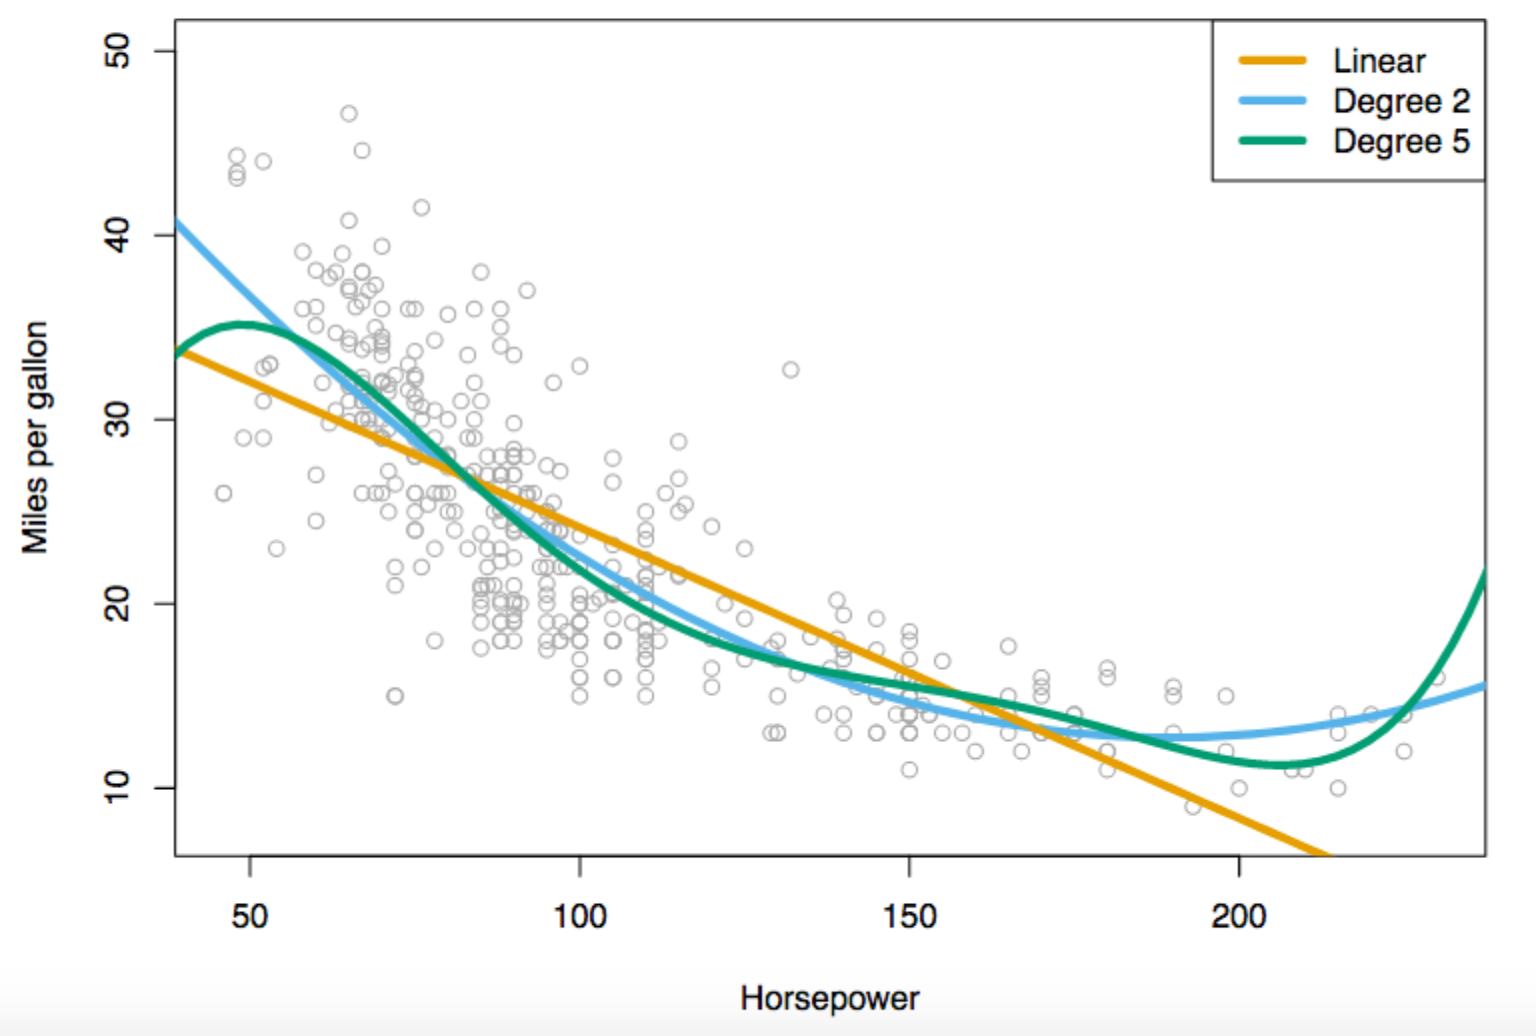
\includegraphics{interpolation_example}

    \subsubsection{Given Linear Test Data}\label{given-linear-training-data}

Knowing that the data represents a linear relationship, a linear fit of
the training data will better predict the test data, decreasing the RSS.
A more flexible model will adapt better to the training data, but the
flexibility will make it difficult to predict new data accurately (test
data). this is illustrated by the green line above. The cubic model will
be swayed by noise in the training data and attempt to fit to it.
Therefore, linear model will be much accurate when new data is
presented, especially if the true relationship is linear

    \subsubsection{Given non-linear Training Data}\label{given-non-linear-training-data}

Again, a more flexible model will preform better (lower RSS) in
training. Because the model is more flexible, it will pass through more
points minimizing RSS until it passes through every point (RSS =0);
however this can be very dangerous, as illustrated by the image above,
the yellow line (linear) under fits, the green line (quintic) overfits.
The blue line most accurately fits the data. Because this data set is
fairly small (1 regressors, 1 predictor, 100 samples), it will be most
beneficial to visualize the data on a 2d plot and pick the regression
that appears to follow the underlying trend of the data. If
visualization is not possible, the cubic model will have a lower RSS.

    \subsubsection{Given Unknown Data}\label{given-unknown-data}

Without visualizing the underlying data it is hard to tell how this will
perform. If the data truly has a cubic relationship, then the cubic fit
will have a lower RSS. For this scenario, I would want to visualize the
data before making a final decision.

    \subsection{RSS proof}\label{rss-proof}

    Let \(\bar{y}\) = the average of all y values

Let \(\bar{x}\) = the average of all x values

Therefore the line y = \(\bar{y}\) minimizes the RSS in the y axis as
shown by the image below: 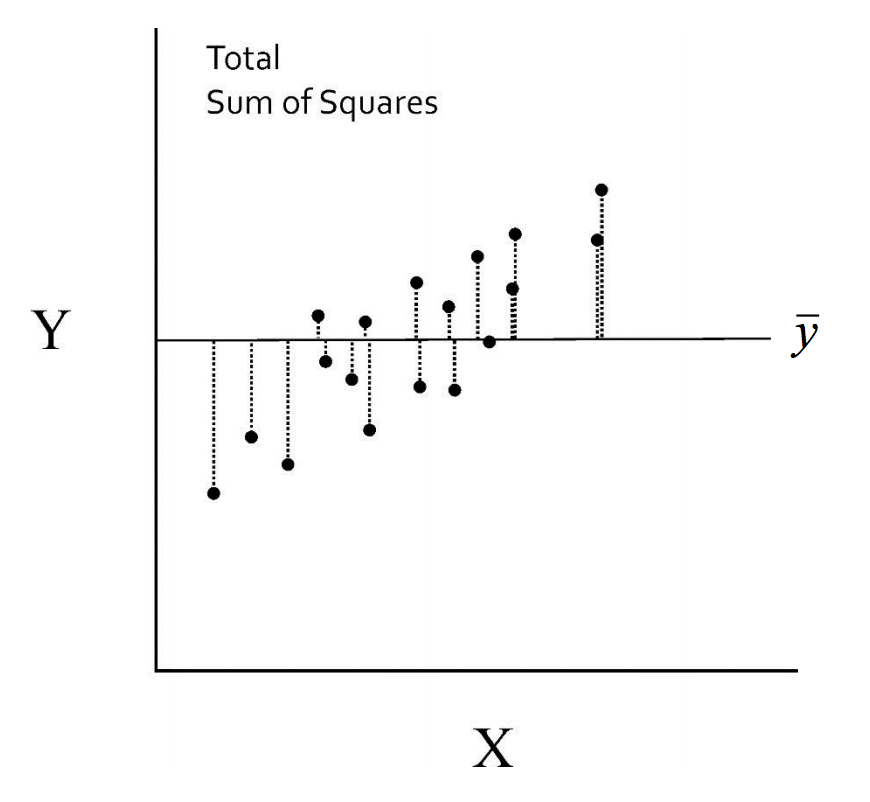
\includegraphics{rssY}

The same logic can be applied for the line x = \(\bar{x}\).

\(\hat{\beta}_1\) computes the slope by determining the covariance of x
and y and normalizing by the x values. This will determine
how best to fit the slope to the set of points.

\(\hat{\beta}_0\) computes the ideal intercept by beginning at the
(\(\bar{x}\), \(\bar{y}\)) and stepping back until x = 0. This will
determine the best intercept.

Therefore, if \(\bar{x}\) and \(\bar{y}\) minimize error on the
respective axis, then to minimize the error for this linear model, the
line should pass through the point (\(\bar{x}\), \(\bar{y}\)). To finish
minimizing error, the line should consider the slope and intercept of
the line as denoted by \(\hat{\beta}_0\) and \(\hat{\beta}_1\)

    

    

    \subsection{Applied}\label{applied}

    \subsection{Fitting linear regression to
data}\label{fitting-linear-regression-to-data}

    \begin{Verbatim}[commandchars=\\\{\}]
{\color{incolor}In [{\color{incolor}2}]:} \PY{k+kn}{import} \PY{n+nn}{numpy} \PY{k}{as} \PY{n+nn}{np}
        \PY{k+kn}{import} \PY{n+nn}{pandas} \PY{k}{as} \PY{n+nn}{pd}
        \PY{k+kn}{import} \PY{n+nn}{seaborn} \PY{k}{as} \PY{n+nn}{sns}
        \PY{k+kn}{import} \PY{n+nn}{matplotlib}\PY{n+nn}{.}\PY{n+nn}{pyplot} \PY{k}{as} \PY{n+nn}{plt}
        \PY{o}{\PYZpc{}}\PY{k}{matplotlib} inline
        \PY{n}{sns}\PY{o}{.}\PY{n}{set}\PY{p}{(}\PY{n}{context}\PY{o}{=}\PY{l+s+s1}{\PYZsq{}}\PY{l+s+s1}{poster}\PY{l+s+s1}{\PYZsq{}}\PY{p}{,} \PY{n}{style}\PY{o}{=}\PY{l+s+s1}{\PYZsq{}}\PY{l+s+s1}{whitegrid}\PY{l+s+s1}{\PYZsq{}}\PY{p}{)}
\end{Verbatim}

    \begin{Verbatim}[commandchars=\\\{\}]
{\color{incolor}In [{\color{incolor}3}]:} \PY{n}{np}\PY{o}{.}\PY{n}{random}\PY{o}{.}\PY{n}{seed}\PY{p}{(}\PY{n}{seed}\PY{o}{=}\PY{l+m+mi}{42}\PY{p}{)}
        \PY{n}{mu}\PY{p}{,} \PY{n}{sigma} \PY{o}{=} \PY{l+m+mi}{0}\PY{p}{,} \PY{l+m+mi}{1}
        \PY{n}{x} \PY{o}{=} \PY{n}{np}\PY{o}{.}\PY{n}{random}\PY{o}{.}\PY{n}{normal}\PY{p}{(}\PY{n}{mu}\PY{p}{,} \PY{n}{sigma}\PY{p}{,} \PY{l+m+mi}{100}\PY{p}{)}
\end{Verbatim}

    \begin{Verbatim}[commandchars=\\\{\}]
{\color{incolor}In [{\color{incolor}4}]:} \PY{n}{np}\PY{o}{.}\PY{n}{random}\PY{o}{.}\PY{n}{seed}\PY{p}{(}\PY{n}{seed}\PY{o}{=}\PY{l+m+mi}{31}\PY{p}{)}
        \PY{n}{eps} \PY{o}{=} \PY{n}{np}\PY{o}{.}\PY{n}{random}\PY{o}{.}\PY{n}{normal}\PY{p}{(}\PY{l+m+mi}{0}\PY{p}{,}\PY{n}{np}\PY{o}{.}\PY{n}{sqrt}\PY{p}{(}\PY{l+m+mf}{0.25}\PY{p}{)}\PY{p}{,} \PY{l+m+mi}{100}\PY{p}{)}
\end{Verbatim}

    \begin{Verbatim}[commandchars=\\\{\}]
{\color{incolor}In [{\color{incolor}5}]:} \PY{n}{Y} \PY{o}{=} \PY{o}{\PYZhy{}}\PY{l+m+mi}{1} \PY{o}{+} \PY{l+m+mf}{0.5}\PY{o}{*}\PY{n}{x} \PY{o}{+} \PY{n}{eps}
\end{Verbatim}

    \begin{Verbatim}[commandchars=\\\{\}]
{\color{incolor}In [{\color{incolor}6}]:} \PY{n}{np}\PY{o}{.}\PY{n}{size}\PY{p}{(}\PY{n}{Y}\PY{p}{)}
\end{Verbatim}

            \begin{Verbatim}[commandchars=\\\{\}]
{\color{outcolor}Out[{\color{outcolor}6}]:} 100
\end{Verbatim}
        
    As indicated above, Y is 100 values long, as expected. \#\#\#\#
\(\beta_0\) = -1 \#\#\#\# \(\beta_1\) = 0.5

    \begin{Verbatim}[commandchars=\\\{\}]
{\color{incolor}In [{\color{incolor}7}]:} \PY{n}{plt}\PY{o}{.}\PY{n}{scatter}\PY{p}{(}\PY{n}{x}\PY{p}{,} \PY{n}{Y}\PY{p}{)}
\end{Verbatim}

            \begin{Verbatim}[commandchars=\\\{\}]
{\color{outcolor}Out[{\color{outcolor}7}]:} <matplotlib.collections.PathCollection at 0x11a0f7278>
\end{Verbatim}
        
    \begin{center}
    \adjustimage{max size={0.9\linewidth}{0.9\paperheight}}{Homework 2_files/Homework 2_24_1.png}
    \end{center}
    { \hspace*{\fill} \\}
    
    I see a relatively linear correlation, as expected, but there is
variation due to the addition of ``noise'' which is generated by
\(\epsilon\).

    \begin{Verbatim}[commandchars=\\\{\}]
{\color{incolor}In [{\color{incolor}8}]:} \PY{k+kn}{from} \PY{n+nn}{sklearn}\PY{n+nn}{.}\PY{n+nn}{linear\PYZus{}model} \PY{k}{import} \PY{n}{LinearRegression}
        \PY{k+kn}{from} \PY{n+nn}{matplotlib}\PY{n+nn}{.}\PY{n+nn}{collections} \PY{k}{import} \PY{n}{LineCollection}
        \PY{k+kn}{from} \PY{n+nn}{sklearn}\PY{n+nn}{.}\PY{n+nn}{metrics} \PY{k}{import} \PY{n}{mean\PYZus{}squared\PYZus{}error}\PY{p}{,} \PY{n}{classification\PYZus{}report}
        \PY{k+kn}{import} \PY{n+nn}{statsmodels}\PY{n+nn}{.}\PY{n+nn}{api} \PY{k}{as} \PY{n+nn}{sm}
        \PY{k+kn}{import} \PY{n+nn}{scipy}\PY{n+nn}{.}\PY{n+nn}{stats} \PY{k}{as} \PY{n+nn}{stats}
\end{Verbatim}

    \begin{Verbatim}[commandchars=\\\{\}]
/Users/Braden/anaconda/lib/python3.6/site-packages/statsmodels/compat/pandas.py:56: FutureWarning: The pandas.core.datetools module is deprecated and will be removed in a future version. Please use the pandas.tseries module instead.
  from pandas.core import datetools

    \end{Verbatim}

    \begin{Verbatim}[commandchars=\\\{\}]
{\color{incolor}In [{\color{incolor}9}]:} \PY{n}{lr} \PY{o}{=} \PY{n}{LinearRegression}\PY{p}{(}\PY{p}{)}
        \PY{n}{lr}\PY{o}{.}\PY{n}{fit}\PY{p}{(}\PY{n}{x}\PY{p}{[}\PY{p}{:}\PY{p}{,} \PY{n}{np}\PY{o}{.}\PY{n}{newaxis}\PY{p}{]}\PY{p}{,} \PY{n}{Y}\PY{p}{)}  \PY{c+c1}{\PYZsh{} x needs to be 2d for LinearRegression}
        \PY{n}{predsLr} \PY{o}{=} \PY{n}{lr}\PY{o}{.}\PY{n}{predict}\PY{p}{(}\PY{n}{x}\PY{p}{[}\PY{p}{:}\PY{p}{,} \PY{n}{np}\PY{o}{.}\PY{n}{newaxis}\PY{p}{]}\PY{p}{)}
\end{Verbatim}

    \begin{Verbatim}[commandchars=\\\{\}]
{\color{incolor}In [{\color{incolor}10}]:} \PY{n+nb}{print}\PY{p}{(}\PY{l+s+s2}{\PYZdq{}}\PY{l+s+s2}{Best Fit: y = }\PY{l+s+s2}{\PYZdq{}} \PY{o}{+} \PY{n+nb}{str}\PY{p}{(}\PY{n}{np}\PY{o}{.}\PY{n}{round}\PY{p}{(}\PY{n}{lr}\PY{o}{.}\PY{n}{coef\PYZus{}}\PY{p}{[}\PY{l+m+mi}{0}\PY{p}{]}\PY{p}{,} \PY{l+m+mi}{3}\PY{p}{)}\PY{p}{)}\PY{o}{+}\PY{l+s+s2}{\PYZdq{}}\PY{l+s+s2}{x }\PY{l+s+s2}{\PYZdq{}} \PY{o}{+}  \PY{n+nb}{str}\PY{p}{(}\PY{n}{np}\PY{o}{.}\PY{n}{round}\PY{p}{(}\PY{n}{lr}\PY{o}{.}\PY{n}{intercept\PYZus{}}\PY{p}{,} \PY{l+m+mi}{3}\PY{p}{)}\PY{p}{)}\PY{p}{)}
         \PY{n+nb}{print}\PY{p}{(}\PY{l+s+s2}{\PYZdq{}}\PY{l+s+s2}{beta\PYZus{}0 = }\PY{l+s+s2}{\PYZdq{}}\PY{o}{+} \PY{n+nb}{str}\PY{p}{(}\PY{n}{np}\PY{o}{.}\PY{n}{round}\PY{p}{(}\PY{n}{lr}\PY{o}{.}\PY{n}{intercept\PYZus{}}\PY{p}{,} \PY{l+m+mi}{3}\PY{p}{)}\PY{p}{)}\PY{p}{)}
         \PY{n+nb}{print}\PY{p}{(}\PY{l+s+s2}{\PYZdq{}}\PY{l+s+s2}{beta\PYZus{}1 = }\PY{l+s+s2}{\PYZdq{}}\PY{o}{+} \PY{n+nb}{str}\PY{p}{(}\PY{n}{np}\PY{o}{.}\PY{n}{round}\PY{p}{(}\PY{n}{lr}\PY{o}{.}\PY{n}{coef\PYZus{}}\PY{p}{[}\PY{l+m+mi}{0}\PY{p}{]}\PY{p}{,} \PY{l+m+mi}{3}\PY{p}{)}\PY{p}{)}\PY{p}{)}
         \PY{n}{RSS} \PY{o}{=} \PY{n}{np}\PY{o}{.}\PY{n}{round}\PY{p}{(}\PY{n}{np}\PY{o}{.}\PY{n}{sum}\PY{p}{(}\PY{p}{(}\PY{n}{Y}\PY{o}{\PYZhy{}}\PY{n}{predsLr}\PY{p}{)}\PY{o}{*}\PY{o}{*}\PY{l+m+mi}{2}\PY{p}{)}\PY{p}{,} \PY{l+m+mi}{4}\PY{p}{)}
         \PY{n}{RSE} \PY{o}{=} \PY{n}{np}\PY{o}{.}\PY{n}{round}\PY{p}{(}\PY{n}{np}\PY{o}{.}\PY{n}{sqrt}\PY{p}{(}\PY{l+m+mi}{1}\PY{o}{/}\PY{n+nb}{len}\PY{p}{(}\PY{n}{Y}\PY{o}{\PYZhy{}}\PY{l+m+mi}{2}\PY{p}{)}\PY{o}{*}\PY{n}{RSS}\PY{p}{)}\PY{p}{,} \PY{l+m+mi}{4}\PY{p}{)}
         \PY{n}{MSE} \PY{o}{=} \PY{n}{np}\PY{o}{.}\PY{n}{round}\PY{p}{(}\PY{n}{mean\PYZus{}squared\PYZus{}error}\PY{p}{(}\PY{n}{Y}\PY{p}{,} \PY{n}{predsLr}\PY{p}{)}\PY{p}{,} \PY{l+m+mi}{4}\PY{p}{)}
         \PY{n+nb}{print}\PY{p}{(}\PY{l+s+s1}{\PYZsq{}}\PY{l+s+s1}{RSS = }\PY{l+s+s1}{\PYZsq{}} \PY{o}{+} \PY{n+nb}{str}\PY{p}{(}\PY{n}{RSS}\PY{p}{)}\PY{p}{)}
         \PY{n+nb}{print}\PY{p}{(}\PY{l+s+s1}{\PYZsq{}}\PY{l+s+s1}{RSE = }\PY{l+s+s1}{\PYZsq{}} \PY{o}{+} \PY{n+nb}{str}\PY{p}{(}\PY{n}{RSE}\PY{p}{)}\PY{p}{)}
         \PY{n+nb}{print}\PY{p}{(}\PY{l+s+s2}{\PYZdq{}}\PY{l+s+s2}{MSE = }\PY{l+s+s2}{\PYZdq{}} \PY{o}{+}  \PY{n+nb}{str}\PY{p}{(}\PY{n}{MSE}\PY{p}{)}\PY{p}{)}
\end{Verbatim}

    \begin{Verbatim}[commandchars=\\\{\}]
Best Fit: y = 0.491x -1.074
beta\_0 = -1.074
beta\_1 = 0.491
RSS = 26.0699
RSE = 0.5106
MSE = 0.2607

    \end{Verbatim}

    \begin{Verbatim}[commandchars=\\\{\}]
{\color{incolor}In [{\color{incolor}11}]:} \PY{n}{results} \PY{o}{=} \PY{n}{sm}\PY{o}{.}\PY{n}{OLS}\PY{p}{(}\PY{n}{Y}\PY{p}{,} \PY{n}{sm}\PY{o}{.}\PY{n}{add\PYZus{}constant}\PY{p}{(}\PY{n}{x}\PY{p}{)}\PY{p}{)}\PY{o}{.}\PY{n}{fit}\PY{p}{(}\PY{p}{)}
         \PY{n+nb}{print}\PY{p}{(}\PY{n}{results}\PY{o}{.}\PY{n}{summary}\PY{p}{(}\PY{p}{)}\PY{p}{)}
\end{Verbatim}

    \begin{Verbatim}[commandchars=\\\{\}]
                            OLS Regression Results                            
==============================================================================
Dep. Variable:                      y   R-squared:                       0.430
Model:                            OLS   Adj. R-squared:                  0.424
Method:                 Least Squares   F-statistic:                     74.02
Date:                Mon, 25 Sep 2017   Prob (F-statistic):           1.29e-13
Time:                        12:14:35   Log-Likelihood:                -74.674
No. Observations:                 100   AIC:                             153.3
Df Residuals:                      98   BIC:                             158.6
Df Model:                           1                                         
Covariance Type:            nonrobust                                         
==============================================================================
                 coef    std err          t      P>|t|      [0.025      0.975]
------------------------------------------------------------------------------
const         -1.0742      0.052    -20.691      0.000      -1.177      -0.971
x1             0.4911      0.057      8.603      0.000       0.378       0.604
==============================================================================
Omnibus:                        3.815   Durbin-Watson:                   2.002
Prob(Omnibus):                  0.148   Jarque-Bera (JB):                3.267
Skew:                           0.431   Prob(JB):                        0.195
Kurtosis:                       3.206   Cond. No.                         1.16
==============================================================================

Warnings:
[1] Standard Errors assume that the covariance matrix of the errors is correctly specified.

    \end{Verbatim}

    Using both linear regression and statsmodels, the coefficients are the
same. \(\hat{\beta}_0 = -1.0742\) and \(\hat{\beta}_1 = 0.4911\). These
vary slightly from the values provided, but not substantially.

    \begin{Verbatim}[commandchars=\\\{\}]
{\color{incolor}In [{\color{incolor}12}]:} \PY{n}{n} \PY{o}{=} \PY{n+nb}{len}\PY{p}{(}\PY{n}{Y}\PY{p}{)}
         
         \PY{n}{segments} \PY{o}{=} \PY{p}{[}\PY{p}{[}\PY{p}{[}\PY{n}{i}\PY{p}{,} \PY{n}{Y}\PY{p}{[}\PY{n}{i}\PY{p}{]}\PY{p}{]}\PY{p}{]} \PY{k}{for} \PY{n}{i} \PY{o+ow}{in} \PY{n+nb}{range}\PY{p}{(}\PY{n}{n}\PY{p}{)}\PY{p}{]}
         \PY{n}{lc} \PY{o}{=} \PY{n}{LineCollection}\PY{p}{(}\PY{n}{segments}\PY{p}{,} \PY{n}{zorder}\PY{o}{=}\PY{l+m+mi}{0}\PY{p}{)}
         \PY{n}{lc}\PY{o}{.}\PY{n}{set\PYZus{}array}\PY{p}{(}\PY{n}{np}\PY{o}{.}\PY{n}{ones}\PY{p}{(}\PY{n+nb}{len}\PY{p}{(}\PY{n}{Y}\PY{p}{)}\PY{p}{)}\PY{p}{)}
         \PY{n}{lc}\PY{o}{.}\PY{n}{set\PYZus{}linewidths}\PY{p}{(}\PY{l+m+mf}{0.5} \PY{o}{*} \PY{n}{np}\PY{o}{.}\PY{n}{ones}\PY{p}{(}\PY{n}{n}\PY{p}{)}\PY{p}{)}
         
         \PY{n}{fig} \PY{o}{=} \PY{n}{plt}\PY{o}{.}\PY{n}{figure}\PY{p}{(}\PY{p}{)}
         \PY{n}{plt}\PY{o}{.}\PY{n}{plot}\PY{p}{(}\PY{n}{x}\PY{p}{,} \PY{n}{Y}\PY{p}{,} \PY{l+s+s1}{\PYZsq{}}\PY{l+s+s1}{r.}\PY{l+s+s1}{\PYZsq{}}\PY{p}{,} \PY{n}{markersize}\PY{o}{=}\PY{l+m+mi}{12}\PY{p}{)}
         \PY{n}{plt}\PY{o}{.}\PY{n}{plot}\PY{p}{(}\PY{n}{x}\PY{p}{,} \PY{n}{results}\PY{o}{.}\PY{n}{fittedvalues}\PY{p}{,} \PY{l+s+s1}{\PYZsq{}}\PY{l+s+s1}{b\PYZhy{}}\PY{l+s+s1}{\PYZsq{}}\PY{p}{)}
         \PY{n}{plt}\PY{o}{.}\PY{n}{gca}\PY{p}{(}\PY{p}{)}\PY{o}{.}\PY{n}{add\PYZus{}collection}\PY{p}{(}\PY{n}{lc}\PY{p}{)}
         \PY{n}{plt}\PY{o}{.}\PY{n}{legend}\PY{p}{(}\PY{p}{(}\PY{l+s+s1}{\PYZsq{}}\PY{l+s+s1}{Data}\PY{l+s+s1}{\PYZsq{}}\PY{p}{,} \PY{l+s+s1}{\PYZsq{}}\PY{l+s+s1}{Linear Fit}\PY{l+s+s1}{\PYZsq{}}\PY{p}{)}\PY{p}{,} \PY{n}{loc}\PY{o}{=}\PY{l+s+s1}{\PYZsq{}}\PY{l+s+s1}{lower right}\PY{l+s+s1}{\PYZsq{}}\PY{p}{)}
         \PY{n}{plt}\PY{o}{.}\PY{n}{title}\PY{p}{(}\PY{l+s+s1}{\PYZsq{}}\PY{l+s+s1}{Linear Best Fit regression}\PY{l+s+s1}{\PYZsq{}}\PY{p}{)}
         \PY{n}{plt}\PY{o}{.}\PY{n}{show}\PY{p}{(}\PY{p}{)}
\end{Verbatim}

    \begin{center}
    \adjustimage{max size={0.9\linewidth}{0.9\paperheight}}{Homework 2_files/Homework 2_31_0.png}
    \end{center}
    { \hspace*{\fill} \\}
    
    \begin{Verbatim}[commandchars=\\\{\}]
{\color{incolor}In [{\color{incolor}13}]:} \PY{n}{X} \PY{o}{=} \PY{n}{np}\PY{o}{.}\PY{n}{column\PYZus{}stack}\PY{p}{(}\PY{p}{(}\PY{p}{(}\PY{n}{x}\PY{p}{)}\PY{o}{*}\PY{o}{*}\PY{l+m+mi}{2}\PY{p}{,} \PY{n}{x}\PY{p}{)}\PY{p}{)}
         \PY{n}{X} \PY{o}{=} \PY{n}{sm}\PY{o}{.}\PY{n}{add\PYZus{}constant}\PY{p}{(}\PY{n}{X}\PY{p}{)}
         \PY{n}{Beta} \PY{o}{=} \PY{n}{np}\PY{o}{.}\PY{n}{polyfit}\PY{p}{(}\PY{n}{x}\PY{p}{,} \PY{n}{Y}\PY{p}{,} \PY{l+m+mi}{2}\PY{p}{)}
         \PY{n}{y} \PY{o}{=} \PY{n}{np}\PY{o}{.}\PY{n}{dot}\PY{p}{(}\PY{n}{X}\PY{p}{,} \PY{n}{Beta}\PY{p}{)} \PY{o}{+} \PY{n}{eps}
         \PY{n}{res} \PY{o}{=} \PY{n}{sm}\PY{o}{.}\PY{n}{OLS}\PY{p}{(}\PY{n}{y}\PY{p}{,}\PY{n}{X}\PY{p}{)}\PY{o}{.}\PY{n}{fit}\PY{p}{(}\PY{p}{)}
         \PY{n+nb}{print}\PY{p}{(}\PY{n}{res}\PY{o}{.}\PY{n}{summary}\PY{p}{(}\PY{p}{)}\PY{p}{)}
\end{Verbatim}

    \begin{Verbatim}[commandchars=\\\{\}]
                            OLS Regression Results                            
==============================================================================
Dep. Variable:                      y   R-squared:                       0.851
Model:                            OLS   Adj. R-squared:                  0.848
Method:                 Least Squares   F-statistic:                     276.1
Date:                Mon, 25 Sep 2017   Prob (F-statistic):           9.06e-41
Time:                        12:14:35   Log-Likelihood:                -74.399
No. Observations:                 100   AIC:                             154.8
Df Residuals:                      97   BIC:                             162.6
Df Model:                           2                                         
Covariance Type:            nonrobust                                         
==============================================================================
                 coef    std err          t      P>|t|      [0.025      0.975]
------------------------------------------------------------------------------
const         -0.0814      0.064     -1.274      0.206      -0.208       0.045
x1             0.4441      0.047      9.445      0.000       0.351       0.537
x2            -1.0686      0.060    -17.885      0.000      -1.187      -0.950
==============================================================================
Omnibus:                        4.045   Durbin-Watson:                   2.001
Prob(Omnibus):                  0.132   Jarque-Bera (JB):                3.508
Skew:                           0.448   Prob(JB):                        0.173
Kurtosis:                       3.200   Cond. No.                         2.27
==============================================================================

Warnings:
[1] Standard Errors assume that the covariance matrix of the errors is correctly specified.

    \end{Verbatim}

    \begin{Verbatim}[commandchars=\\\{\}]
{\color{incolor}In [{\color{incolor}14}]:} \PY{n}{q} \PY{o}{=} \PY{n}{np}\PY{o}{.}\PY{n}{poly1d}\PY{p}{(}\PY{n}{Beta}\PY{p}{)}
         \PY{n}{xp} \PY{o}{=} \PY{n}{np}\PY{o}{.}\PY{n}{linspace}\PY{p}{(}\PY{n+nb}{min}\PY{p}{(}\PY{n}{x}\PY{p}{)}\PY{p}{,} \PY{n+nb}{max}\PY{p}{(}\PY{n}{x}\PY{p}{)}\PY{p}{,} \PY{l+m+mi}{100}\PY{p}{)}
\end{Verbatim}

    \begin{Verbatim}[commandchars=\\\{\}]
{\color{incolor}In [{\color{incolor}15}]:} \PY{n}{y\PYZus{}pred} \PY{o}{=} \PY{n}{res}\PY{o}{.}\PY{n}{params}\PY{p}{[}\PY{l+m+mi}{0}\PY{p}{]}\PY{o}{*}\PY{p}{(}\PY{n}{xp}\PY{o}{*}\PY{o}{*}\PY{l+m+mi}{2}\PY{p}{)} \PY{o}{+} \PY{n}{res}\PY{o}{.}\PY{n}{params}\PY{p}{[}\PY{l+m+mi}{1}\PY{p}{]}\PY{o}{*}\PY{n}{xp} \PY{o}{+} \PY{n}{res}\PY{o}{.}\PY{n}{params}\PY{p}{[}\PY{l+m+mi}{2}\PY{p}{]}
\end{Verbatim}

    \begin{Verbatim}[commandchars=\\\{\}]
{\color{incolor}In [{\color{incolor}16}]:} \PY{n}{plt}\PY{o}{.}\PY{n}{plot}\PY{p}{(}\PY{n}{x}\PY{p}{,} \PY{n}{Y}\PY{p}{,} \PY{l+s+s1}{\PYZsq{}}\PY{l+s+s1}{.}\PY{l+s+s1}{\PYZsq{}}\PY{p}{,} \PY{n}{xp}\PY{p}{,} \PY{n}{q}\PY{p}{(}\PY{n}{xp}\PY{p}{)}\PY{p}{,} \PY{l+s+s1}{\PYZsq{}}\PY{l+s+s1}{\PYZhy{}}\PY{l+s+s1}{\PYZsq{}}\PY{p}{,} \PY{n}{xp}\PY{p}{,} \PY{n}{y\PYZus{}pred}\PY{p}{,} \PY{l+s+s1}{\PYZsq{}}\PY{l+s+s1}{\PYZhy{}\PYZhy{}}\PY{l+s+s1}{\PYZsq{}}\PY{p}{)}
         \PY{n}{plt}\PY{o}{.}\PY{n}{legend}\PY{p}{(}\PY{p}{[}\PY{l+s+s1}{\PYZsq{}}\PY{l+s+s1}{Data}\PY{l+s+s1}{\PYZsq{}}\PY{p}{,} \PY{l+s+s1}{\PYZsq{}}\PY{l+s+s1}{Numpy Polyplot}\PY{l+s+s1}{\PYZsq{}}\PY{p}{,} \PY{l+s+s1}{\PYZsq{}}\PY{l+s+s1}{OSL Reg}\PY{l+s+s1}{\PYZsq{}}\PY{p}{]}\PY{p}{)}
\end{Verbatim}

            \begin{Verbatim}[commandchars=\\\{\}]
{\color{outcolor}Out[{\color{outcolor}16}]:} <matplotlib.legend.Legend at 0x11ea71ef0>
\end{Verbatim}
        
    \begin{center}
    \adjustimage{max size={0.9\linewidth}{0.9\paperheight}}{Homework 2_files/Homework 2_35_1.png}
    \end{center}
    { \hspace*{\fill} \\}
    
    ****Why are these values diffrent?

    \begin{Verbatim}[commandchars=\\\{\}]
{\color{incolor}In [{\color{incolor}17}]:} \PY{n}{var} \PY{o}{=} \PY{p}{[}\PY{o}{.}\PY{l+m+mi}{125}\PY{p}{,} \PY{o}{.}\PY{l+m+mi}{25}\PY{p}{,} \PY{o}{.}\PY{l+m+mi}{375}\PY{p}{,} \PY{o}{.}\PY{l+m+mi}{125}\PY{p}{,} \PY{o}{.}\PY{l+m+mi}{25}\PY{p}{,} \PY{o}{.}\PY{l+m+mi}{375}\PY{p}{]}
         \PY{n}{model} \PY{o}{=} \PY{p}{[}\PY{l+s+s1}{\PYZsq{}}\PY{l+s+s1}{Linear}\PY{l+s+s1}{\PYZsq{}}\PY{p}{,} \PY{l+s+s1}{\PYZsq{}}\PY{l+s+s1}{Linear}\PY{l+s+s1}{\PYZsq{}}\PY{p}{,} \PY{l+s+s1}{\PYZsq{}}\PY{l+s+s1}{Linear}\PY{l+s+s1}{\PYZsq{}}\PY{p}{,} \PY{l+s+s1}{\PYZsq{}}\PY{l+s+s1}{Quad}\PY{l+s+s1}{\PYZsq{}}\PY{p}{,} \PY{l+s+s1}{\PYZsq{}}\PY{l+s+s1}{Quad}\PY{l+s+s1}{\PYZsq{}}\PY{p}{,} \PY{l+s+s1}{\PYZsq{}}\PY{l+s+s1}{Quad}\PY{l+s+s1}{\PYZsq{}}\PY{p}{]}
         \PY{n}{df} \PY{o}{=} \PY{n}{pd}\PY{o}{.}\PY{n}{DataFrame}\PY{p}{(}\PY{n}{np}\PY{o}{.}\PY{n}{zeros}\PY{p}{(}\PY{p}{[}\PY{l+m+mi}{6}\PY{p}{,} \PY{l+m+mi}{12}\PY{p}{]}\PY{p}{)}\PY{p}{,} \PY{n}{columns} \PY{o}{=} 
                           \PY{p}{[}\PY{l+s+s1}{\PYZsq{}}\PY{l+s+s1}{Eps Var}\PY{l+s+s1}{\PYZsq{}}\PY{p}{,} \PY{l+s+s1}{\PYZsq{}}\PY{l+s+s1}{Model}\PY{l+s+s1}{\PYZsq{}}\PY{p}{,} \PY{l+s+s1}{\PYZsq{}}\PY{l+s+s1}{RSS}\PY{l+s+s1}{\PYZsq{}}\PY{p}{,} \PY{l+s+s1}{\PYZsq{}}\PY{l+s+s1}{MSE}\PY{l+s+s1}{\PYZsq{}}\PY{p}{,} \PY{l+s+s1}{\PYZsq{}}\PY{l+s+s1}{RSE}\PY{l+s+s1}{\PYZsq{}}\PY{p}{,} \PY{l+s+s1}{\PYZsq{}}\PY{l+s+s1}{b1}\PY{l+s+s1}{\PYZsq{}}\PY{p}{,} \PY{l+s+s1}{\PYZsq{}}\PY{l+s+s1}{b2}\PY{l+s+s1}{\PYZsq{}}\PY{p}{,} \PY{l+s+s1}{\PYZsq{}}\PY{l+s+s1}{Int}\PY{l+s+s1}{\PYZsq{}}\PY{p}{,} \PY{l+s+s1}{\PYZsq{}}\PY{l+s+s1}{ci [b2,b1,int]}\PY{l+s+s1}{\PYZsq{}}\PY{p}{,}
                           \PY{l+s+s1}{\PYZsq{}}\PY{l+s+s1}{Std Err b2}\PY{l+s+s1}{\PYZsq{}}\PY{p}{,} \PY{l+s+s1}{\PYZsq{}}\PY{l+s+s1}{Std Err b1}\PY{l+s+s1}{\PYZsq{}}\PY{p}{,} \PY{l+s+s1}{\PYZsq{}}\PY{l+s+s1}{Std Err b0}\PY{l+s+s1}{\PYZsq{}}\PY{p}{]}\PY{p}{)}
         \PY{n}{df}\PY{p}{[}\PY{l+s+s1}{\PYZsq{}}\PY{l+s+s1}{Eps Var}\PY{l+s+s1}{\PYZsq{}}\PY{p}{]} \PY{o}{=} \PY{n}{var}
         \PY{n}{df}\PY{p}{[}\PY{l+s+s1}{\PYZsq{}}\PY{l+s+s1}{Model}\PY{l+s+s1}{\PYZsq{}}\PY{p}{]} \PY{o}{=} \PY{n}{model}
         \PY{n}{np}\PY{o}{.}\PY{n}{random}\PY{o}{.}\PY{n}{seed}\PY{p}{(}\PY{n}{seed}\PY{o}{=}\PY{l+m+mi}{31}\PY{p}{)}
         
         \PY{n}{X} \PY{o}{=} \PY{n}{np}\PY{o}{.}\PY{n}{column\PYZus{}stack}\PY{p}{(}\PY{p}{(}\PY{p}{(}\PY{n}{x}\PY{p}{)}\PY{o}{*}\PY{o}{*}\PY{l+m+mi}{2}\PY{p}{,} \PY{n}{x}\PY{p}{,} \PY{n}{np}\PY{o}{.}\PY{n}{ones}\PY{p}{(}\PY{p}{[}\PY{l+m+mi}{100}\PY{p}{,}\PY{l+m+mi}{1}\PY{p}{]}\PY{p}{)}\PY{p}{)}\PY{p}{)}
         \PY{n}{xp} \PY{o}{=} \PY{n}{np}\PY{o}{.}\PY{n}{linspace}\PY{p}{(}\PY{n+nb}{min}\PY{p}{(}\PY{n}{x}\PY{p}{)}\PY{p}{,} \PY{n+nb}{max}\PY{p}{(}\PY{n}{x}\PY{p}{)}\PY{p}{,} \PY{l+m+mi}{100}\PY{p}{)}
         
         \PY{n}{f}\PY{p}{,} \PY{p}{(}\PY{n}{ax1}\PY{p}{,} \PY{n}{ax2}\PY{p}{,} \PY{n}{ax3}\PY{p}{)} \PY{o}{=} \PY{n}{plt}\PY{o}{.}\PY{n}{subplots}\PY{p}{(}\PY{l+m+mi}{1}\PY{p}{,} \PY{l+m+mi}{3}\PY{p}{,} \PY{n}{sharey}\PY{o}{=}\PY{k+kc}{True}\PY{p}{,} \PY{n}{sharex}\PY{o}{=}\PY{k+kc}{True}\PY{p}{)}
         
         \PY{k}{for} \PY{n}{i} \PY{o+ow}{in} \PY{n}{df}\PY{o}{.}\PY{n}{index}\PY{p}{:}
             \PY{n}{v} \PY{o}{=} \PY{n}{df}\PY{p}{[}\PY{l+s+s1}{\PYZsq{}}\PY{l+s+s1}{Eps Var}\PY{l+s+s1}{\PYZsq{}}\PY{p}{]}\PY{p}{[}\PY{n}{i}\PY{p}{]}
             \PY{n}{eps} \PY{o}{=} \PY{n}{np}\PY{o}{.}\PY{n}{random}\PY{o}{.}\PY{n}{normal}\PY{p}{(}\PY{l+m+mi}{0}\PY{p}{,}\PY{n}{np}\PY{o}{.}\PY{n}{sqrt}\PY{p}{(}\PY{n}{v}\PY{p}{)}\PY{p}{,} \PY{l+m+mi}{100}\PY{p}{)}
             \PY{n}{Y} \PY{o}{=} \PY{o}{\PYZhy{}}\PY{l+m+mi}{1} \PY{o}{+} \PY{l+m+mf}{0.5}\PY{o}{*}\PY{n}{x} \PY{o}{+} \PY{n}{eps}
             \PY{k}{if} \PY{l+s+s1}{\PYZsq{}}\PY{l+s+s1}{Linear}\PY{l+s+s1}{\PYZsq{}} \PY{o+ow}{in} \PY{n}{df}\PY{p}{[}\PY{l+s+s1}{\PYZsq{}}\PY{l+s+s1}{Model}\PY{l+s+s1}{\PYZsq{}}\PY{p}{]}\PY{p}{[}\PY{n}{i}\PY{p}{]}\PY{p}{:}
                 \PY{n}{m} \PY{o}{=} \PY{n}{sm}\PY{o}{.}\PY{n}{OLS}\PY{p}{(}\PY{n}{Y}\PY{p}{,}\PY{n}{sm}\PY{o}{.}\PY{n}{add\PYZus{}constant}\PY{p}{(}\PY{n}{x}\PY{p}{)}\PY{p}{)}\PY{o}{.}\PY{n}{fit}\PY{p}{(}\PY{p}{)}
                 \PY{n}{df}\PY{o}{.}\PY{n}{set\PYZus{}value}\PY{p}{(}\PY{n}{i}\PY{p}{,} \PY{p}{[}\PY{l+s+s1}{\PYZsq{}}\PY{l+s+s1}{b1}\PY{l+s+s1}{\PYZsq{}}\PY{p}{,} \PY{l+s+s1}{\PYZsq{}}\PY{l+s+s1}{Int}\PY{l+s+s1}{\PYZsq{}}\PY{p}{]}\PY{p}{,} \PY{n}{m}\PY{o}{.}\PY{n}{params}\PY{p}{)}
                 \PY{n}{df}\PY{o}{.}\PY{n}{set\PYZus{}value}\PY{p}{(}\PY{n}{i}\PY{p}{,} \PY{p}{[}\PY{l+s+s1}{\PYZsq{}}\PY{l+s+s1}{RSS}\PY{l+s+s1}{\PYZsq{}}\PY{p}{]}\PY{p}{,} \PY{n}{np}\PY{o}{.}\PY{n}{round}\PY{p}{(}\PY{n}{m}\PY{o}{.}\PY{n}{ssr}\PY{p}{,} \PY{l+m+mi}{4}\PY{p}{)}\PY{p}{)}
                 \PY{n}{df}\PY{o}{.}\PY{n}{set\PYZus{}value}\PY{p}{(}\PY{n}{i}\PY{p}{,} \PY{p}{[}\PY{l+s+s1}{\PYZsq{}}\PY{l+s+s1}{MSE}\PY{l+s+s1}{\PYZsq{}}\PY{p}{]}\PY{p}{,} \PY{n}{np}\PY{o}{.}\PY{n}{round}\PY{p}{(}\PY{n}{m}\PY{o}{.}\PY{n}{mse\PYZus{}resid}\PY{p}{,} \PY{l+m+mi}{4}\PY{p}{)}\PY{p}{)}
                 \PY{n}{df}\PY{o}{.}\PY{n}{set\PYZus{}value}\PY{p}{(}\PY{n}{i}\PY{p}{,} \PY{p}{[}\PY{l+s+s1}{\PYZsq{}}\PY{l+s+s1}{RSE}\PY{l+s+s1}{\PYZsq{}}\PY{p}{]}\PY{p}{,} \PY{n}{np}\PY{o}{.}\PY{n}{round}\PY{p}{(}\PY{n}{np}\PY{o}{.}\PY{n}{sqrt}\PY{p}{(}\PY{l+m+mi}{1}\PY{o}{/}\PY{n+nb}{len}\PY{p}{(}\PY{n}{Y}\PY{o}{\PYZhy{}}\PY{l+m+mi}{2}\PY{p}{)}\PY{o}{*}\PY{n}{m}\PY{o}{.}\PY{n}{ssr}\PY{p}{)}\PY{p}{,} \PY{l+m+mi}{4}\PY{p}{)}\PY{p}{)}
                 \PY{n}{df}\PY{o}{.}\PY{n}{set\PYZus{}value}\PY{p}{(}\PY{n}{i}\PY{p}{,} \PY{p}{[}\PY{l+s+s1}{\PYZsq{}}\PY{l+s+s1}{Std Err b1}\PY{l+s+s1}{\PYZsq{}}\PY{p}{,} \PY{l+s+s1}{\PYZsq{}}\PY{l+s+s1}{Std Err b0}\PY{l+s+s1}{\PYZsq{}}\PY{p}{]}\PY{p}{,} \PY{n}{np}\PY{o}{.}\PY{n}{round}\PY{p}{(}\PY{n}{m}\PY{o}{.}\PY{n}{bse}\PY{p}{,} \PY{l+m+mi}{4} \PY{p}{)}\PY{p}{)}
                 \PY{n}{df}\PY{o}{.}\PY{n}{set\PYZus{}value}\PY{p}{(}\PY{n}{i}\PY{p}{,} \PY{p}{[}\PY{l+s+s1}{\PYZsq{}}\PY{l+s+s1}{ci [b2,b1,int]}\PY{l+s+s1}{\PYZsq{}}\PY{p}{]}\PY{p}{,} \PY{n+nb}{str}\PY{p}{(}\PY{n}{np}\PY{o}{.}\PY{n}{round}\PY{p}{(}\PY{n}{m}\PY{o}{.}\PY{n}{conf\PYZus{}int}\PY{p}{(}\PY{p}{)}\PY{p}{,} \PY{l+m+mi}{4}\PY{p}{)}\PY{p}{)}\PY{p}{)}
                 
                 \PY{k}{if} \PY{n}{v} \PY{o}{==} \PY{o}{.}\PY{l+m+mi}{375}\PY{p}{:}
                     \PY{k}{if} \PY{n}{i} \PY{o}{\PYZlt{}} \PY{l+m+mi}{3}\PY{p}{:}
                         \PY{n}{ax3}\PY{o}{.}\PY{n}{plot}\PY{p}{(}\PY{n}{x}\PY{p}{,} \PY{n}{Y}\PY{p}{,} \PY{l+s+s1}{\PYZsq{}}\PY{l+s+s1}{.}\PY{l+s+s1}{\PYZsq{}}\PY{p}{,} \PY{n}{label}\PY{o}{=}\PY{l+s+s1}{\PYZsq{}}\PY{l+s+s1}{Data}\PY{l+s+s1}{\PYZsq{}}\PY{p}{)}
                     \PY{n}{ax3}\PY{o}{.}\PY{n}{plot}\PY{p}{(}\PY{n}{x}\PY{p}{,} \PY{n}{m}\PY{o}{.}\PY{n}{fittedvalues}\PY{p}{,} \PY{l+s+s1}{\PYZsq{}}\PY{l+s+s1}{\PYZhy{}}\PY{l+s+s1}{\PYZsq{}}\PY{p}{,} \PY{n}{label}\PY{o}{=}\PY{l+s+s1}{\PYZsq{}}\PY{l+s+s1}{Linear}\PY{l+s+s1}{\PYZsq{}}\PY{p}{)}
                 \PY{k}{elif} \PY{n}{v} \PY{o}{==} \PY{o}{.}\PY{l+m+mi}{25} \PY{o+ow}{and} \PY{n}{i} \PY{o}{\PYZlt{}} \PY{l+m+mi}{3}\PY{p}{:}
                     \PY{k}{if} \PY{n}{i} \PY{o}{\PYZlt{}} \PY{l+m+mi}{3}\PY{p}{:}
                         \PY{n}{ax2}\PY{o}{.}\PY{n}{plot}\PY{p}{(}\PY{n}{x}\PY{p}{,} \PY{n}{Y}\PY{p}{,} \PY{l+s+s1}{\PYZsq{}}\PY{l+s+s1}{.}\PY{l+s+s1}{\PYZsq{}}\PY{p}{,} \PY{n}{label}\PY{o}{=}\PY{l+s+s1}{\PYZsq{}}\PY{l+s+s1}{Data}\PY{l+s+s1}{\PYZsq{}}\PY{p}{)}
                     \PY{n}{ax2}\PY{o}{.}\PY{n}{plot}\PY{p}{(}\PY{n}{x}\PY{p}{,} \PY{n}{m}\PY{o}{.}\PY{n}{fittedvalues}\PY{p}{,} \PY{l+s+s1}{\PYZsq{}}\PY{l+s+s1}{\PYZhy{}}\PY{l+s+s1}{\PYZsq{}}\PY{p}{,} \PY{n}{label}\PY{o}{=}\PY{l+s+s1}{\PYZsq{}}\PY{l+s+s1}{Linear}\PY{l+s+s1}{\PYZsq{}}\PY{p}{)}
                 \PY{k}{else}\PY{p}{:}
                     \PY{k}{if} \PY{n}{i} \PY{o}{\PYZlt{}} \PY{l+m+mi}{3}\PY{p}{:}
                         \PY{n}{ax1}\PY{o}{.}\PY{n}{plot}\PY{p}{(}\PY{n}{x}\PY{p}{,} \PY{n}{Y}\PY{p}{,} \PY{l+s+s1}{\PYZsq{}}\PY{l+s+s1}{.}\PY{l+s+s1}{\PYZsq{}}\PY{p}{,} \PY{n}{label}\PY{o}{=}\PY{l+s+s1}{\PYZsq{}}\PY{l+s+s1}{Data}\PY{l+s+s1}{\PYZsq{}}\PY{p}{)}
                     \PY{n}{ax1}\PY{o}{.}\PY{n}{plot}\PY{p}{(}\PY{n}{x}\PY{p}{,} \PY{n}{m}\PY{o}{.}\PY{n}{fittedvalues}\PY{p}{,} \PY{l+s+s1}{\PYZsq{}}\PY{l+s+s1}{\PYZhy{}}\PY{l+s+s1}{\PYZsq{}}\PY{p}{,} \PY{n}{label}\PY{o}{=}\PY{l+s+s1}{\PYZsq{}}\PY{l+s+s1}{Linear}\PY{l+s+s1}{\PYZsq{}}\PY{p}{)}
                     
             \PY{k}{else}\PY{p}{:}
                 \PY{n}{Beta} \PY{o}{=} \PY{n}{np}\PY{o}{.}\PY{n}{polyfit}\PY{p}{(}\PY{n}{x}\PY{p}{,} \PY{n}{Y}\PY{p}{,} \PY{l+m+mi}{2}\PY{p}{)}
                 \PY{n}{y} \PY{o}{=} \PY{n}{np}\PY{o}{.}\PY{n}{dot}\PY{p}{(}\PY{n}{X}\PY{p}{,} \PY{n}{Beta}\PY{p}{)} \PY{o}{+} \PY{n}{eps}
                 \PY{n}{m} \PY{o}{=} \PY{n}{sm}\PY{o}{.}\PY{n}{OLS}\PY{p}{(}\PY{n}{y}\PY{p}{,}\PY{n}{X}\PY{p}{)}\PY{o}{.}\PY{n}{fit}\PY{p}{(}\PY{p}{)}        
                 \PY{n}{df}\PY{o}{.}\PY{n}{set\PYZus{}value}\PY{p}{(}\PY{n}{i}\PY{p}{,} \PY{p}{[}\PY{l+s+s1}{\PYZsq{}}\PY{l+s+s1}{b2}\PY{l+s+s1}{\PYZsq{}}\PY{p}{,}\PY{l+s+s1}{\PYZsq{}}\PY{l+s+s1}{b1}\PY{l+s+s1}{\PYZsq{}}\PY{p}{,} \PY{l+s+s1}{\PYZsq{}}\PY{l+s+s1}{Int}\PY{l+s+s1}{\PYZsq{}}\PY{p}{]}\PY{p}{,} \PY{n}{m}\PY{o}{.}\PY{n}{params}\PY{p}{)}
                 \PY{n}{df}\PY{o}{.}\PY{n}{set\PYZus{}value}\PY{p}{(}\PY{n}{i}\PY{p}{,} \PY{p}{[}\PY{l+s+s1}{\PYZsq{}}\PY{l+s+s1}{RSS}\PY{l+s+s1}{\PYZsq{}}\PY{p}{]}\PY{p}{,} \PY{n}{np}\PY{o}{.}\PY{n}{round}\PY{p}{(}\PY{n}{m}\PY{o}{.}\PY{n}{ssr}\PY{p}{,} \PY{l+m+mi}{4}\PY{p}{)}\PY{p}{)}
                 \PY{n}{df}\PY{o}{.}\PY{n}{set\PYZus{}value}\PY{p}{(}\PY{n}{i}\PY{p}{,} \PY{p}{[}\PY{l+s+s1}{\PYZsq{}}\PY{l+s+s1}{MSE}\PY{l+s+s1}{\PYZsq{}}\PY{p}{]}\PY{p}{,} \PY{n}{np}\PY{o}{.}\PY{n}{round}\PY{p}{(}\PY{n}{m}\PY{o}{.}\PY{n}{mse\PYZus{}resid}\PY{p}{,} \PY{l+m+mi}{4}\PY{p}{)}\PY{p}{)}
                 \PY{n}{df}\PY{o}{.}\PY{n}{set\PYZus{}value}\PY{p}{(}\PY{n}{i}\PY{p}{,} \PY{p}{[}\PY{l+s+s1}{\PYZsq{}}\PY{l+s+s1}{RSE}\PY{l+s+s1}{\PYZsq{}}\PY{p}{]}\PY{p}{,} \PY{n}{np}\PY{o}{.}\PY{n}{round}\PY{p}{(}\PY{n}{np}\PY{o}{.}\PY{n}{sqrt}\PY{p}{(}\PY{l+m+mi}{1}\PY{o}{/}\PY{n+nb}{len}\PY{p}{(}\PY{n}{Y}\PY{o}{\PYZhy{}}\PY{l+m+mi}{2}\PY{p}{)}\PY{o}{*}\PY{n}{m}\PY{o}{.}\PY{n}{ssr}\PY{p}{)}\PY{p}{,} \PY{l+m+mi}{4}\PY{p}{)}\PY{p}{)}
                 \PY{n}{df}\PY{o}{.}\PY{n}{set\PYZus{}value}\PY{p}{(}\PY{n}{i}\PY{p}{,} \PY{p}{[}\PY{l+s+s1}{\PYZsq{}}\PY{l+s+s1}{Std Err b2}\PY{l+s+s1}{\PYZsq{}}\PY{p}{,} \PY{l+s+s1}{\PYZsq{}}\PY{l+s+s1}{Std Err b1}\PY{l+s+s1}{\PYZsq{}}\PY{p}{,} \PY{l+s+s1}{\PYZsq{}}\PY{l+s+s1}{Std Err b0}\PY{l+s+s1}{\PYZsq{}}\PY{p}{]}\PY{p}{,} \PY{n}{np}\PY{o}{.}\PY{n}{round}\PY{p}{(}\PY{n}{m}\PY{o}{.}\PY{n}{bse}\PY{p}{,} \PY{l+m+mi}{4} \PY{p}{)}\PY{p}{)}
                 \PY{n}{df}\PY{o}{.}\PY{n}{set\PYZus{}value}\PY{p}{(}\PY{n}{i}\PY{p}{,} \PY{p}{[}\PY{l+s+s1}{\PYZsq{}}\PY{l+s+s1}{ci [b2,b1,int]}\PY{l+s+s1}{\PYZsq{}}\PY{p}{]}\PY{p}{,} \PY{n+nb}{str}\PY{p}{(}\PY{n}{np}\PY{o}{.}\PY{n}{round}\PY{p}{(}\PY{n}{m}\PY{o}{.}\PY{n}{conf\PYZus{}int}\PY{p}{(}\PY{p}{)}\PY{p}{,} \PY{l+m+mi}{4}\PY{p}{)}\PY{p}{)}\PY{p}{)}
                 \PY{n}{y\PYZus{}pred} \PY{o}{=} \PY{n}{m}\PY{o}{.}\PY{n}{params}\PY{p}{[}\PY{l+m+mi}{0}\PY{p}{]}\PY{o}{*}\PY{p}{(}\PY{n}{xp}\PY{o}{*}\PY{o}{*}\PY{l+m+mi}{2}\PY{p}{)} \PY{o}{+} \PY{n}{m}\PY{o}{.}\PY{n}{params}\PY{p}{[}\PY{l+m+mi}{1}\PY{p}{]}\PY{o}{*}\PY{n}{xp} \PY{o}{+} \PY{n}{m}\PY{o}{.}\PY{n}{params}\PY{p}{[}\PY{l+m+mi}{2}\PY{p}{]}
                 \PY{k}{if} \PY{n}{v} \PY{o}{==} \PY{o}{.}\PY{l+m+mi}{375}\PY{p}{:}
                     \PY{n}{l3} \PY{o}{=} \PY{n}{ax3}\PY{o}{.}\PY{n}{plot}\PY{p}{(}\PY{n}{xp}\PY{p}{,} \PY{n}{y\PYZus{}pred}\PY{p}{,} \PY{n}{label}\PY{o}{=}\PY{l+s+s1}{\PYZsq{}}\PY{l+s+s1}{Quadratic}\PY{l+s+s1}{\PYZsq{}}\PY{p}{)}
                 \PY{k}{elif} \PY{n}{v} \PY{o}{==} \PY{o}{.}\PY{l+m+mi}{25}\PY{p}{:}
                     \PY{n}{l3} \PY{o}{=} \PY{n}{ax2}\PY{o}{.}\PY{n}{plot}\PY{p}{(}\PY{n}{xp}\PY{p}{,} \PY{n}{y\PYZus{}pred}\PY{p}{,} \PY{n}{label}\PY{o}{=}\PY{l+s+s1}{\PYZsq{}}\PY{l+s+s1}{Quadratic}\PY{l+s+s1}{\PYZsq{}}\PY{p}{)}
                 \PY{k}{else}\PY{p}{:}
                     \PY{n}{l3} \PY{o}{=} \PY{n}{ax1}\PY{o}{.}\PY{n}{plot}\PY{p}{(}\PY{n}{xp}\PY{p}{,} \PY{n}{y\PYZus{}pred}\PY{p}{,} \PY{n}{label}\PY{o}{=}\PY{l+s+s1}{\PYZsq{}}\PY{l+s+s1}{Quadratic}\PY{l+s+s1}{\PYZsq{}}\PY{p}{)}
         
         \PY{n}{handles}\PY{p}{,} \PY{n}{labels} \PY{o}{=} \PY{n}{ax3}\PY{o}{.}\PY{n}{get\PYZus{}legend\PYZus{}handles\PYZus{}labels}\PY{p}{(}\PY{p}{)}
         \PY{n}{f}\PY{o}{.}\PY{n}{legend}\PY{p}{(}\PY{n}{handles}\PY{p}{,} \PY{n}{labels}\PY{p}{,} \PY{n}{loc} \PY{o}{=} \PY{p}{(}\PY{l+m+mf}{0.5}\PY{p}{,} \PY{l+m+mi}{0}\PY{p}{)}\PY{p}{,} \PY{n}{ncol}\PY{o}{=}\PY{l+m+mi}{5} \PY{p}{)}
\end{Verbatim}

            \begin{Verbatim}[commandchars=\\\{\}]
{\color{outcolor}Out[{\color{outcolor}17}]:} <matplotlib.legend.Legend at 0x11f094860>
\end{Verbatim}
        
    \begin{center}
    \adjustimage{max size={0.9\linewidth}{0.9\paperheight}}{Homework 2_files/Homework 2_37_1.png}
    \end{center}
    { \hspace*{\fill} \\}
    
    \begin{Verbatim}[commandchars=\\\{\}]
{\color{incolor}In [{\color{incolor}18}]:} \PY{n}{df}
\end{Verbatim}

            \begin{Verbatim}[commandchars=\\\{\}]
{\color{outcolor}Out[{\color{outcolor}18}]:}    Eps Var   Model      RSS     MSE     RSE        b1        b2       Int  \textbackslash{}
         0    0.125  Linear  13.0350  0.1330  0.3610 -1.052466  0.000000  0.493682   
         1    0.250  Linear  22.1979  0.2265  0.4711 -1.038366  0.000000  0.505778   
         2    0.375  Linear  39.5935  0.4040  0.6292 -0.994353  0.000000  0.435533   
         3    0.125    Quad  15.1892  0.1566  0.3897  0.412405 -0.062746 -1.044036   
         4    0.250    Quad  22.1001  0.2278  0.4701  0.321515  0.085363 -0.989854   
         5    0.375    Quad  34.4266  0.3549  0.5867  0.202061 -0.214669 -0.665325   
         
                                               ci [b2,b1,int]  Std Err b2  Std Err b1  \textbackslash{}
         0            [[-1.1253 -0.9796]\textbackslash{}n [ 0.4136  0.5738]]      0.0000      0.0367   
         1            [[-1.1334 -0.9433]\textbackslash{}n [ 0.4013  0.6103]]      0.0000      0.0479   
         2            [[-1.1213 -0.8674]\textbackslash{}n [ 0.2959  0.5751]]      0.0000      0.0640   
         3  [[-0.1342  0.0087]\textbackslash{}n [ 0.3216  0.5032]\textbackslash{}n [-1.1{\ldots}      0.0360      0.0457   
         4  [[ -8.00000000e-04   1.71500000e-01]\textbackslash{}n [  2.12{\ldots}      0.0434      0.0552   
         5  [[-0.3222 -0.1071]\textbackslash{}n [ 0.0654  0.3387]\textbackslash{}n [-0.8{\ldots}      0.0542      0.0688   
         
            Std Err b0  
         0      0.0404  
         1      0.0527  
         2      0.0703  
         3      0.0489  
         4      0.0590  
         5      0.0737  
\end{Verbatim}
        
    \begin{Verbatim}[commandchars=\\\{\}]
{\color{incolor}In [{\color{incolor}19}]:} \PY{n}{sns}\PY{o}{.}\PY{n}{pairplot}\PY{p}{(}\PY{n}{df}\PY{p}{,} \PY{n}{hue}\PY{o}{=}\PY{l+s+s1}{\PYZsq{}}\PY{l+s+s1}{Model}\PY{l+s+s1}{\PYZsq{}}\PY{p}{)}
\end{Verbatim}

            \begin{Verbatim}[commandchars=\\\{\}]
{\color{outcolor}Out[{\color{outcolor}19}]:} <seaborn.axisgrid.PairGrid at 0x11ed909b0>
\end{Verbatim}
        
    \begin{center}
    \adjustimage{max size={0.9\linewidth}{0.9\paperheight}}{Homework 2_files/Homework 2_39_1.png}
    \end{center}
    { \hspace*{\fill} \\}
    
    This has generated fairly expected resaults. When the varience of
eplison decreased, linear models tended to preform better. This is
indicated by the RSS, MSE, and RSE.

    \begin{Verbatim}[commandchars=\\\{\}]
{\color{incolor}In [{\color{incolor}20}]:} \PY{n}{df}\PY{p}{[}\PY{p}{[}\PY{l+s+s1}{\PYZsq{}}\PY{l+s+s1}{Eps Var}\PY{l+s+s1}{\PYZsq{}}\PY{p}{,} \PY{l+s+s1}{\PYZsq{}}\PY{l+s+s1}{Model}\PY{l+s+s1}{\PYZsq{}}\PY{p}{,} \PY{l+s+s1}{\PYZsq{}}\PY{l+s+s1}{ci [b2,b1,int]}\PY{l+s+s1}{\PYZsq{}}\PY{p}{,} \PY{l+s+s1}{\PYZsq{}}\PY{l+s+s1}{Std Err b2}\PY{l+s+s1}{\PYZsq{}}\PY{p}{,} \PY{l+s+s1}{\PYZsq{}}\PY{l+s+s1}{Std Err b1}\PY{l+s+s1}{\PYZsq{}}\PY{p}{,} \PY{l+s+s1}{\PYZsq{}}\PY{l+s+s1}{Std Err b0}\PY{l+s+s1}{\PYZsq{}}\PY{p}{]}\PY{p}{]}
\end{Verbatim}

            \begin{Verbatim}[commandchars=\\\{\}]
{\color{outcolor}Out[{\color{outcolor}20}]:}    Eps Var   Model                                     ci [b2,b1,int]  \textbackslash{}
         0    0.125  Linear            [[-1.1253 -0.9796]\textbackslash{}n [ 0.4136  0.5738]]   
         1    0.250  Linear            [[-1.1334 -0.9433]\textbackslash{}n [ 0.4013  0.6103]]   
         2    0.375  Linear            [[-1.1213 -0.8674]\textbackslash{}n [ 0.2959  0.5751]]   
         3    0.125    Quad  [[-0.1342  0.0087]\textbackslash{}n [ 0.3216  0.5032]\textbackslash{}n [-1.1{\ldots}   
         4    0.250    Quad  [[ -8.00000000e-04   1.71500000e-01]\textbackslash{}n [  2.12{\ldots}   
         5    0.375    Quad  [[-0.3222 -0.1071]\textbackslash{}n [ 0.0654  0.3387]\textbackslash{}n [-0.8{\ldots}   
         
            Std Err b2  Std Err b1  Std Err b0  
         0      0.0000      0.0367      0.0404  
         1      0.0000      0.0479      0.0527  
         2      0.0000      0.0640      0.0703  
         3      0.0360      0.0457      0.0489  
         4      0.0434      0.0552      0.0590  
         5      0.0542      0.0688      0.0737  
\end{Verbatim}
        
    \subsubsection{Confidence intervals:}\label{confidence-intervals}

The confidence intervals appears smaller on models with lower error.
This is expected as the model is more likely to contain the true value
of the data if there is less varience. To minimize confidence intervals,
our sample size would need to increase substantially. This is indicated
by the Central Limit Theory Proof.

    \subsection{Question 6}\label{question-6}

    \begin{Verbatim}[commandchars=\\\{\}]
{\color{incolor}In [{\color{incolor}21}]:} \PY{n}{df} \PY{o}{=} \PY{n}{pd}\PY{o}{.}\PY{n}{read\PYZus{}csv}\PY{p}{(}\PY{l+s+s1}{\PYZsq{}}\PY{l+s+s1}{Auto.csv}\PY{l+s+s1}{\PYZsq{}}\PY{p}{)}
\end{Verbatim}

    \begin{Verbatim}[commandchars=\\\{\}]
{\color{incolor}In [{\color{incolor}22}]:} \PY{n}{df}\PY{o}{.}\PY{n}{head}\PY{p}{(}\PY{p}{)}
\end{Verbatim}

            \begin{Verbatim}[commandchars=\\\{\}]
{\color{outcolor}Out[{\color{outcolor}22}]:}     mpg  cylinders  displacement  horsepower  weight  acceleration  year  \textbackslash{}
         0  18.0          8         307.0         130    3504          12.0    70   
         1  15.0          8         350.0         165    3693          11.5    70   
         2  18.0          8         318.0         150    3436          11.0    70   
         3  16.0          8         304.0         150    3433          12.0    70   
         4  17.0          8         302.0         140    3449          10.5    70   
         
            origin                       name  
         0       1  chevrolet chevelle malibu  
         1       1          buick skylark 320  
         2       1         plymouth satellite  
         3       1              amc rebel sst  
         4       1                ford torino  
\end{Verbatim}
        
    \begin{Verbatim}[commandchars=\\\{\}]
{\color{incolor}In [{\color{incolor} }]:} \PY{n}{df}\PY{o}{.}\PY{n}{info}\PY{p}{(}\PY{p}{)}
\end{Verbatim}

    \begin{Verbatim}[commandchars=\\\{\}]
<class 'pandas.core.frame.DataFrame'>
RangeIndex: 392 entries, 0 to 391
Data columns (total 9 columns):
mpg             392 non-null float64
cylinders       392 non-null int64
displacement    392 non-null float64
horsepower      392 non-null int64
weight          392 non-null int64
acceleration    392 non-null float64
year            392 non-null int64
origin          392 non-null int64
name            392 non-null object
dtypes: float64(3), int64(5), object(1)
memory usage: 27.6+ KB

    \end{Verbatim}

    \begin{Verbatim}[commandchars=\\\{\}]
{\color{incolor}In [{\color{incolor} }]:} \PY{n}{sns}\PY{o}{.}\PY{n}{pairplot}\PY{p}{(}\PY{n}{df}\PY{p}{,} \PY{n}{hue}\PY{o}{=}\PY{l+s+s1}{\PYZsq{}}\PY{l+s+s1}{origin}\PY{l+s+s1}{\PYZsq{}}\PY{p}{)}
\end{Verbatim}

    \begin{Verbatim}[commandchars=\\\{\}]
{\color{incolor}In [{\color{incolor} }]:} \PY{n}{p} \PY{o}{=} \PY{n}{sns}\PY{o}{.}\PY{n}{heatmap}\PY{p}{(}\PY{n}{df}\PY{o}{.}\PY{n}{corr}\PY{p}{(}\PY{p}{)}\PY{p}{,} \PY{n}{annot}\PY{o}{=}\PY{k+kc}{True}\PY{p}{)}
        \PY{n}{plt}\PY{o}{.}\PY{n}{xticks}\PY{p}{(}\PY{n}{rotation}\PY{o}{=}\PY{l+m+mi}{90}\PY{p}{)} 
\end{Verbatim}

    \begin{Verbatim}[commandchars=\\\{\}]
{\color{incolor}In [{\color{incolor} }]:} \PY{k+kn}{from} \PY{n+nn}{statsmodels}\PY{n+nn}{.}\PY{n+nn}{formula}\PY{n+nn}{.}\PY{n+nn}{api} \PY{k}{import} \PY{n}{ols}
        
        \PY{n}{res} \PY{o}{=} \PY{n}{ols}\PY{p}{(}\PY{n}{formula}\PY{o}{=}\PY{l+s+s1}{\PYZsq{}}\PY{l+s+s1}{mpg \PYZti{} cylinders + displacement + horsepower + weight + acceleration + year + origin}\PY{l+s+s1}{\PYZsq{}}\PY{p}{,} 
                     \PY{n}{data}\PY{o}{=}\PY{n}{df}\PY{p}{)}\PY{o}{.}\PY{n}{fit}\PY{p}{(}\PY{p}{)}
        \PY{n+nb}{print}\PY{p}{(}\PY{n}{res}\PY{o}{.}\PY{n}{summary}\PY{p}{(}\PY{p}{)}\PY{p}{)}
\end{Verbatim}

    \begin{Verbatim}[commandchars=\\\{\}]
{\color{incolor}In [{\color{incolor} }]:} \PY{n}{RSS} \PY{o}{=} \PY{n}{np}\PY{o}{.}\PY{n}{round}\PY{p}{(}\PY{n}{res}\PY{o}{.}\PY{n}{ssr}\PY{p}{,} \PY{l+m+mi}{4}\PY{p}{)}
        \PY{n}{RSE} \PY{o}{=} \PY{n}{np}\PY{o}{.}\PY{n}{round}\PY{p}{(}\PY{n}{np}\PY{o}{.}\PY{n}{sqrt}\PY{p}{(}\PY{l+m+mi}{1}\PY{o}{/}\PY{n+nb}{len}\PY{p}{(}\PY{n}{Y}\PY{o}{\PYZhy{}}\PY{l+m+mi}{2}\PY{p}{)}\PY{o}{*}\PY{n}{RSS}\PY{p}{)}\PY{p}{,} \PY{l+m+mi}{4}\PY{p}{)}
        \PY{n}{MSE} \PY{o}{=} \PY{n}{np}\PY{o}{.}\PY{n}{round}\PY{p}{(}\PY{n}{res}\PY{o}{.}\PY{n}{mse\PYZus{}resid}\PY{p}{,} \PY{l+m+mi}{4}\PY{p}{)}
        \PY{n+nb}{print}\PY{p}{(}\PY{l+s+s1}{\PYZsq{}}\PY{l+s+s1}{RSS = }\PY{l+s+s1}{\PYZsq{}} \PY{o}{+} \PY{n+nb}{str}\PY{p}{(}\PY{n}{RSS}\PY{p}{)}\PY{p}{)}
        \PY{n+nb}{print}\PY{p}{(}\PY{l+s+s1}{\PYZsq{}}\PY{l+s+s1}{RSE = }\PY{l+s+s1}{\PYZsq{}} \PY{o}{+} \PY{n+nb}{str}\PY{p}{(}\PY{n}{RSE}\PY{p}{)}\PY{p}{)}
        \PY{n+nb}{print}\PY{p}{(}\PY{l+s+s2}{\PYZdq{}}\PY{l+s+s2}{MSE = }\PY{l+s+s2}{\PYZdq{}} \PY{o}{+}  \PY{n+nb}{str}\PY{p}{(}\PY{n}{MSE}\PY{p}{)}\PY{p}{)}
\end{Verbatim}

    \paragraph{There does appear to be a statistical correlation between the
factors and mpg. More specifically, the intercept, weight, displacement,
year, and origin have the largest impact. This data is highly unlikely
to have ocurred randomly. Logically, as regulations have required car
companies to increase their avergae MPG, year and has a large impact on
MPG. Holding everything else constant, MPG increases by 0.75 for year. I
find it interesting that origin also has a significant impact. Given the
key, it shows that the rest of the world (not America) is much more
efficient than the US. Japan and the EU have much higher MPG
requirements.}\label{there-does-appear-to-be-a-statistical-correlation-between-the-factors-and-mpg.-more-specifically-the-intercept-weight-displacement-year-and-origin-have-the-largest-impact.-this-data-is-highly-unlikely-to-have-ocurred-randomly.-logically-as-regulations-have-required-car-companies-to-increase-their-avergae-mpg-year-and-has-a-large-impact-on-mpg.-holding-everything-else-constant-mpg-increases-by-0.75-for-year.-i-find-it-interesting-that-origin-also-has-a-significant-impact.-given-the-key-it-shows-that-the-rest-of-the-world-not-america-is-much-more-efficient-than-the-us.-japan-and-the-eu-have-much-higher-mpg-requirements.}

    \begin{Verbatim}[commandchars=\\\{\}]
{\color{incolor}In [{\color{incolor} }]:} \PY{n}{plt}\PY{o}{.}\PY{n}{stem}\PY{p}{(}\PY{n}{res}\PY{o}{.}\PY{n}{resid}\PY{p}{)}
        \PY{n}{plt}\PY{o}{.}\PY{n}{title}\PY{p}{(}\PY{l+s+s1}{\PYZsq{}}\PY{l+s+s1}{Stemplot of Residuals}\PY{l+s+s1}{\PYZsq{}}\PY{p}{)}
\end{Verbatim}

    \begin{Verbatim}[commandchars=\\\{\}]
{\color{incolor}In [{\color{incolor} }]:} \PY{n}{sm}\PY{o}{.}\PY{n}{qqplot}\PY{p}{(}\PY{n}{res}\PY{o}{.}\PY{n}{resid}\PY{p}{,} \PY{n}{line}\PY{o}{=}\PY{l+s+s1}{\PYZsq{}}\PY{l+s+s1}{r}\PY{l+s+s1}{\PYZsq{}}\PY{p}{,} \PY{n}{fit}\PY{o}{=}\PY{k+kc}{True}\PY{p}{)}
\end{Verbatim}

    \begin{Verbatim}[commandchars=\\\{\}]
{\color{incolor}In [{\color{incolor} }]:} \PY{n}{sns}\PY{o}{.}\PY{n}{boxplot}\PY{p}{(}\PY{n}{res}\PY{o}{.}\PY{n}{resid}\PY{p}{)}
        \PY{n}{plt}\PY{o}{.}\PY{n}{title}\PY{p}{(}\PY{l+s+s1}{\PYZsq{}}\PY{l+s+s1}{Boxplot of Residuals}\PY{l+s+s1}{\PYZsq{}}\PY{p}{)}
\end{Verbatim}

    It appears that there are outliers. The majority of the model's
residuals appear to fit well to a normal model (as expected) until we
reach the higher and lower quartiles. The Q-Q plot is fitted to a normal
model.

    \subsubsection{Alter Variables by sqrt}\label{alter-variables-by-sqrt}

    \begin{Verbatim}[commandchars=\\\{\}]
{\color{incolor}In [{\color{incolor} }]:} \PY{n}{sqr} \PY{o}{=} \PY{n}{ols}\PY{p}{(}\PY{n}{formula}\PY{o}{=}\PY{l+s+s1}{\PYZsq{}}\PY{l+s+s1}{mpg \PYZti{} cylinders + displacement + horsepower + weight + acceleration + year + origin}\PY{l+s+s1}{\PYZsq{}}\PY{p}{,} 
                     \PY{n}{data}\PY{o}{=}\PY{n}{df}\PY{p}{)}\PY{o}{.}\PY{n}{fit}\PY{p}{(}\PY{p}{)}
        \PY{n}{fig}\PY{p}{,} \PY{p}{[}\PY{n}{ax1}\PY{p}{,} \PY{n}{ax2}\PY{p}{]} \PY{o}{=} \PY{n}{plt}\PY{o}{.}\PY{n}{subplots}\PY{p}{(}\PY{l+m+mi}{1}\PY{p}{,} \PY{l+m+mi}{2}\PY{p}{)}
        \PY{n}{sns}\PY{o}{.}\PY{n}{boxplot}\PY{p}{(}\PY{n}{sqr}\PY{o}{.}\PY{n}{resid}\PY{p}{,} \PY{n}{ax}\PY{o}{=}\PY{n}{ax1}\PY{p}{)}
        \PY{n}{sm}\PY{o}{.}\PY{n}{qqplot}\PY{p}{(}\PY{n}{sqr}\PY{o}{.}\PY{n}{resid}\PY{p}{,} \PY{n}{line}\PY{o}{=}\PY{l+s+s1}{\PYZsq{}}\PY{l+s+s1}{r}\PY{l+s+s1}{\PYZsq{}}\PY{p}{,} \PY{n}{fit}\PY{o}{=}\PY{k+kc}{True}\PY{p}{,} \PY{n}{ax}\PY{o}{=}\PY{n}{ax2}\PY{p}{)}
\end{Verbatim}

    \begin{Verbatim}[commandchars=\\\{\}]
{\color{incolor}In [{\color{incolor} }]:} \PY{n+nb}{print}\PY{p}{(}\PY{n}{sqr}\PY{o}{.}\PY{n}{summary}\PY{p}{(}\PY{p}{)}\PY{p}{)}
\end{Verbatim}

    Sqrt does not appear to deal with the outliers well. I was hoping that
it would minimize the extreme values, but it only enlarged them.

    \subsubsection{Alter Variables by log}\label{alter-variables-by-log}

    \begin{Verbatim}[commandchars=\\\{\}]
{\color{incolor}In [{\color{incolor} }]:} \PY{n}{dflog} \PY{o}{=} \PY{n}{df}\PY{o}{.}\PY{n}{drop}\PY{p}{(}\PY{p}{[}\PY{l+s+s1}{\PYZsq{}}\PY{l+s+s1}{name}\PY{l+s+s1}{\PYZsq{}}\PY{p}{,} \PY{l+s+s1}{\PYZsq{}}\PY{l+s+s1}{mpg}\PY{l+s+s1}{\PYZsq{}}\PY{p}{]}\PY{p}{,} \PY{n}{axis}\PY{o}{=}\PY{l+m+mi}{1}\PY{p}{)}\PY{o}{.}\PY{n}{apply}\PY{p}{(}\PY{n}{np}\PY{o}{.}\PY{n}{log}\PY{p}{)}
        \PY{n}{log} \PY{o}{=} \PY{n}{ols}\PY{p}{(}\PY{n}{formula}\PY{o}{=}\PY{l+s+s1}{\PYZsq{}}\PY{l+s+s1}{mpg \PYZti{} cylinders + displacement + horsepower + weight + acceleration + year + origin}\PY{l+s+s1}{\PYZsq{}}\PY{p}{,} 
                     \PY{n}{data}\PY{o}{=}\PY{n}{pd}\PY{o}{.}\PY{n}{concat}\PY{p}{(}\PY{p}{[}\PY{n}{dflog}\PY{p}{,} \PY{n}{df}\PY{o}{.}\PY{n}{mpg}\PY{p}{]}\PY{p}{,} \PY{n}{axis}\PY{o}{=}\PY{l+m+mi}{1}\PY{p}{)}\PY{p}{)}\PY{o}{.}\PY{n}{fit}\PY{p}{(}\PY{p}{)}
        \PY{n}{fig}\PY{p}{,} \PY{p}{[}\PY{n}{ax1}\PY{p}{,} \PY{n}{ax2}\PY{p}{]} \PY{o}{=} \PY{n}{plt}\PY{o}{.}\PY{n}{subplots}\PY{p}{(}\PY{l+m+mi}{1}\PY{p}{,} \PY{l+m+mi}{2}\PY{p}{)}
        \PY{n}{sns}\PY{o}{.}\PY{n}{boxplot}\PY{p}{(}\PY{n}{log}\PY{o}{.}\PY{n}{resid}\PY{p}{,} \PY{n}{ax}\PY{o}{=}\PY{n}{ax1}\PY{p}{)}
        \PY{n}{sm}\PY{o}{.}\PY{n}{qqplot}\PY{p}{(}\PY{n}{log}\PY{o}{.}\PY{n}{resid}\PY{p}{,} \PY{n}{line}\PY{o}{=}\PY{l+s+s1}{\PYZsq{}}\PY{l+s+s1}{s}\PY{l+s+s1}{\PYZsq{}}\PY{p}{,} \PY{n}{fit}\PY{o}{=}\PY{k+kc}{True}\PY{p}{,} \PY{n}{ax}\PY{o}{=}\PY{n}{ax2}\PY{p}{)}
\end{Verbatim}

    \begin{Verbatim}[commandchars=\\\{\}]
{\color{incolor}In [{\color{incolor} }]:} 
\end{Verbatim}


    % Add a bibliography block to the postdoc
    
    
    
    \end{document}
